\documentclass{article}

% For PDF, suitable for double-sided printing, change the PrintVersion variable below to "true" and use this \documentclass line instead of the one above:
%\documentclass[letterpaper,12pt,titlepage,openright,twoside,final]{book}
\newcommand{\package}[1]{\textbf{#1}} % package names in bold text
\newcommand{\cmmd}[1]{\textbackslash\texttt{#1}} % command name in tt font 
\newcommand{\href}[1]{#1} % does nothing, but defines the command so the print-optimized version will ignore \href tags (redefined by hyperref pkg).
%\newcommand{\texorpdfstring}[2]{#1} % does nothing, but defines the command
% Anything defined here may be redefined by packages added below...

% This package allows if-then-else control structures.
\usepackage{ifthen}
\newboolean{PrintVersion}
\setboolean{PrintVersion}{false}
% CHANGE THIS VALUE TO "true" as necessary, to improve printed results for hard copies by overriding some options of the hyperref package, called below.

%\usepackage{nomencl} % For a nomenclature (optional; available from ctan.org)
\usepackage{amsmath,amssymb,amstext} % Lots of math symbols and environments
\usepackage[pdftex]{graphicx} % For including graphics N.B. pdftex graphics driver
\usepackage{amsmath,amssymb,amstext,amsthm,amsfonts}
\usepackage{dsfont}
\usepackage[pdftex]{graphicx}
\usepackage{caption}
\usepackage{color}% Include colors for document elements
\usepackage{dcolumn}% Align table columns on decimal point
\usepackage{bm}% bold math
\usepackage{float}
\usepackage{multirow}
\usepackage[round]{natbib}   % omit 'round' option for square brackets

\usepackage{algorithm} % For counting chapters
\usepackage{algorithmicx, algpseudocode}
%\renewcommand{\algorithmiccomment}[1]{// #1} % Brackets are confused with the sets
%\algsetup{linenosize=\scriptsize}

% N.B. HYPERREF MUST BE THE LAST PACKAGE LOADED; ADD ADDITIONAL PKGS ABOVE
\usepackage[pdftex,pagebackref=false]{hyperref} % with basic options
%\usepackage[pdftex,pagebackref=true]{hyperref}
% N.B. pagebackref=true provides links back from the References to the body text. This can cause trouble for printing.
% define colours
\definecolor{background-color}{gray}{0.98}
\definecolor{steelblue}{rgb}{0.27, 0.51, 0.71}
\definecolor{brickred}{rgb}{0.8, 0.25, 0.33}
\definecolor{bluegray}{rgb}{0.4, 0.6, 0.8}
\definecolor{amethyst}{rgb}{0.6, 0.4, 0.8}

\hypersetup{
	plainpages=false,       % needed if Roman numbers in frontpages
	unicode=false,          % non-Latin characters in Acrobat's bookmarks
	pdftoolbar=true,        % show Acrobats toolbar?
	pdfmenubar=true,        % show Acrobat's menu?
	pdffitwindow=false,     % window fit to page when opened
	pdfstartview={FitH},    % fits the width of the page to the window
	pdftitle={Genetic Model},    % title: CHANGE THIS TEXT!
	pdfauthor={Chris Salahub},    % author: CHANGE THIS TEXT! and uncomment this line
	%pdfsubject={Statistics},  % subject: CHANGE THIS TEXT! and uncomment this line
	%    pdfkeywords={keyword1} {key2} {key3}, % list of keywords, and uncomment this line if desired
	pdfnewwindow=true,      % links in new window
	colorlinks=true,        % false: boxed links; true: colored links
	linkcolor=steelblue,         % color of internal links
	citecolor=brickred,        % color of links to bibliography
	filecolor=magenta,      % color of file links
	urlcolor=cyan           % color of external links
}
\ifthenelse{\boolean{PrintVersion}}{   % for improved print quality, change some hyperref options
	\hypersetup{	% override some previously defined hyperref options
		%    colorlinks,%
		citecolor=black,%
		filecolor=black,%
		linkcolor=black,%
		urlcolor=black}
}{} % end of ifthenelse (no else)

%\usepackage[automake,toc,abbreviations]{glossaries-extra} % Exception to the rule of hyperref being the last add-on package

% Page margins
% uWaterloo thesis requirements specify a minimum of 1 inch (72pt) margin at the
% top, bottom, and outside page edges and a 1.125 in. (81pt) gutter margin (on binding side). 
\setlength{\marginparwidth}{0pt} % width of margin notes
% N.B. If margin notes are used, you must adjust \textwidth, \marginparwidth
% and \marginparsep so that the space left between the margin notes and page
% edge is less than 15 mm (0.6 in.)
\setlength{\marginparsep}{0pt} % width of space between body text and margin notes
\setlength{\evensidemargin}{0.125in} % Adds 1/8 in. to binding side of all even pages when "twoside" is selected
\setlength{\oddsidemargin}{0.125in} % Adds 1/8 in. to the left of all pages when "oneside" is selected,
% and to the left of all odd pages when "twoside" is selected
\setlength{\textwidth}{6.375in} % assuming US letter paper (8.5 in. x 11 in.) and margins as above
\raggedbottom

\setlength{\parskip}{\medskipamount} % space between paragraphs
\renewcommand{\baselinestretch}{1} % line space setting

% Commands
% Code
\newcommand{\code}[1]{\texttt{#1}}
\newcommand*{\Rnsp}{\textsf{R}}
\newcommand*{\R}{\textsf{R}$~$}
\newcommand*{\Pythonnsp}{\textsf{Python}}
\newcommand*{\Python}{\textsf{Python}$~$}
\newcommand{\pkg}[1]{\textsf{#1}}
\newcommand{\pkgsp}[1]{\textsf{#1}$~$}
\algblock{Input}{EndInput}
\algnotext{EndInput}
\newcommand{\Desc}[2]{\State \makebox[2em][l]{#1}#2}

% Theorem styles
\newtheorem{definition}{Definition}
\newtheorem{theorem}{Theorem}

% vectors
\newcommand{\ve}[1]{\mathbf{#1}}           % for vectors
\newcommand{\sv}[1]{\boldsymbol{#1}}   % for greek letters
\newcommand{\m}[1]{\mathbf{#1}}               % for matrices
\newcommand{\sm}[1]{\boldsymbol{#1}}   % for greek letters
\newcommand{\tr}[1]{{#1}^{\mkern-1.5mu\mathsf{T}}}              % for transpose
\newcommand{\conj}[1]{{#1}^{\ast}}
\newcommand{\norm}[1]{||{#1}||}              % norm
\newcommand{\frob}[1]{\norm{#1}_F}
\newcommand{\abs}[1]{\lvert{#1}\rvert}              % norm
\newcommand*{\mvec}{\operatorname{vec}}
\newcommand*{\trace}{\operatorname{trace}}
\newcommand*{\rank}{\operatorname{rank}}
\newcommand*{\diag}{\operatorname{diag}}
\newcommand*{\vspan}{\operatorname{span}}
\newcommand*{\rowsp}{\operatorname{rowsp}}
\newcommand*{\colsp}{\operatorname{colsp}}
\newcommand*{\svd}{\operatorname{svd}}
\newcommand*{\edm}{\operatorname{edm}}  % euclidean distance matrix (D * D)
\newcommand{\oneblock}[3]{\m{B}_{#1:#2:#3}}
\newcommand{\stripe}[2]{\m{S}_{#1,#2}}

% contingency tables
\newcommand{\abdiff}{\delta_{AB}}

% statistical
\newcommand{\widebar}[1]{\overline{#1}}  
\newcommand{\wig}[1]{\tilde{#1}}  
\newcommand{\bigwig}[1]{\widetilde{#1}}  
\newcommand{\follows}{\sim}  
\newcommand{\leftgiven}{~\left\lvert~}
\newcommand{\given}{~\vert~}
\newcommand{\biggiven}{~\vline~}
\newcommand{\indep}{\bot\hspace{-.6em}\bot}
\newcommand{\notindep}{\bot\hspace{-.6em}\bot\hspace{-0.75em}/\hspace{.4em}}
\newcommand{\depend}{\Join}
\newcommand{\notdepend}{\Join\hspace{-0.9 em}/\hspace{.4em}}
\newcommand{\imply}{\Longrightarrow}
\newcommand{\notimply}{\Longrightarrow \hspace{-1.5em}/ \hspace{0.8em}}
\newcommand{\xyAssociation}{g}
\newcommand{\xDomain}{\mathcal{X}}
\newcommand{\yDomain}{\mathcal{Y}}
\newcommand{\measureRange}{\mathcal{R}}
\newcommand{\bigChi}{\mathcal{D}}
\newcommand{\ind}[2]{I_{#2} \left( #1 \right)}
%\newcommand{\ind}[1]{\mathds{1} \hspace{-0.1cm}\left( #1 \right)}
\newcommand{\mutInf}{\mathcal{I}}

% operators
\newcommand{\Had}{\circ}
\newcommand{\measureAssociation}{G}
\DeclareMathOperator*{\lmin}{Minimize}
\DeclareMathOperator*{\argmin}{arg\,min}
\DeclareMathOperator*{\argmax}{arg\,max}
\DeclareMathOperator*{\arginf}{arg\,inf}
\DeclareMathOperator*{\argsup}{arg\,sup}

% Sets
\newcommand*{\intersect}{\cap}
\newcommand*{\union}{\cup}
\let\oldemptyset\emptyset
\let\emptyset\varnothing

% Fields, Reals, etc. etc
\newcommand{\field}[1]{\mathbb{#1}}
\newcommand{\Reals}{\field{R}}
\newcommand{\Integers}{\field{Z}}
\newcommand{\Naturals}{\field{N}}
\newcommand{\Complex}{\field{C}}
\newcommand{\Rationals}{\field{Q}}

% Editorial
\newcommand{\needtocite}[1]{{\color{red} [Need to cite {#1} here]}}
\newcommand{\comment}[1]{{\color{steelblue} COMMENT:  {#1}}}
\newcommand{\TODO}[1]{{\color{brickred} TODO:  {#1}}}

\title{A structural genetic model to derive map distances and correlation and compare these to reality}
\author{Chris Salahub \\
	\textit{University of Waterloo}}

\begin{document}
	
\maketitle

\begin{abstract}
A structural model of the genome incorporating a modern understanding of the genome and common practice in modern genome-wide association studies is devised. This model demonstrates that the Haldane map distance is a direct consequence of the structure of the genome as it is understood today under reasonable assumptions. The model also supports an analytical derivation of linkage disequilibrium, which is then compared to real data resulting from the BSB mouse cross. A novel plot, the correlation test plot, facilitates this comparison and indicates a close agreement of the model and reality despite simplistic assumptions. Chromosome 4 displays noteworthy departures which warrant further investigation.
\end{abstract}

\section{Introduction} \label{sec:intro}

Genetic research today routinely considers the entirety of a \emph{genome}, defined by \cite{doergeetal1997search} as all heritable material potentially passed from parent to offspring, to identify genetic regions strongly related to measured physical traits. The goal is to associate measured genome sequences, the \emph{genotype}, with physical characteristics, the \emph{phenotype}. Computational and methodological advances in the pursuit of these \emph{quantitative trait loci} (QTLs) have distinguished \emph{genomics} as its own field. Central to genomics is the \emph{genome-wide association study} (GWAS), where many \emph{markers}, sequences of nucleotides at known positions on the genome, are measured. Extracting useful results from markers and measured traits is a complicated task which has motivated decades of statistical and biological research. Interested individuals must sort through this voluminous research in order to understand genomics.

\begin{figure}[!ht]
  \begin{center}
  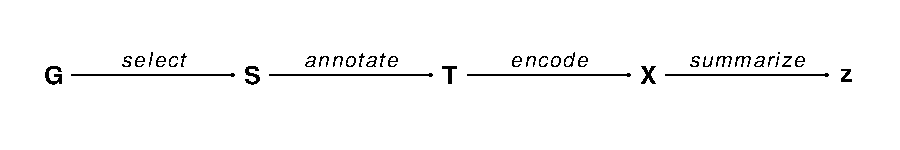
\includegraphics[scale = 1]{./img/modelDiagram.pdf}
  \caption{A structural model of genomic studies.}
  \label{fig:modelDiagram}
\end{center}
\end{figure}

To aid in this, Figure \ref{fig:modelDiagram} draws on the literature to present a structural model of the process of converting raw marker measurements into a form which can be used to identify QTLs. It identifies four key steps (\emph{selection}, \emph{annotation}, \emph{encoding}, and \emph{summarization}) between five increasingly abstract representations of the genome. By highlighting these steps and abstractions in plain language, this model provides a clear map to guide the understanding of GWAS. While it is no replacement surveys such as \cite{uffelmannetal2021gwas, tametal2019benefits} or the literature they outline, it supplies a guiding structural framework with exceptional explanatory power to facilitate understanding of other papers in the field.

The model starts with $\m{G}$, the whole genome of an individual organism. Genetic information is stored in DNA, a long molecule consisting of a sequence of four \emph{nucleotide bases}: guanine, cytosine, adenine, and thymine. A \emph{diplodic} individual inherits one version or \emph{variant} of a complete DNA sequence from each parent, and so has two copies in all \emph{somatic} (i.e. non-reproductive) cells. Though it can be represented as one long sequence, DNA is actually structured into \emph{chromosomes}, separate strands of DNA which contain only a part of the sequence. As most genetic research concerns diplodic species, this is implicitly assumed.

It is usually not feasible or desirable to design a study around the measurement of all of $\m{G}$, and so the \emph{select} step chooses regions to measure. These regions are represented in $\m{S}$. Often $\m{S}$ consists of a series of \emph{single nucleotide polymorphisms} (SNPs), single nucleotide substitutions in a known sequence at a known position. In human studies this is supported by SNP databases such as \cite{NCBIdbSNP} which document hundreds of millions of common SNPs in the human genome. Only a small proportion of these are estimated to occur frequently enough in the population to be useful in a GWAS, perhaps 15 million according to \cite{koboldtetal2013next}. Modern SNP arrays can simultaneously identify roughly one million of these per array, see \cite{laframboise2009, tametal2019benefits}, and most GWAS will measure only one array of SNPs. \emph{Linkage disequilibrium}, effectively the correlation between regions of the genome, facilitates inference to regions outside of those selected in $\m{S}$. While third generation genome sequencing technologies allow for entire genomes to be sequenced, as noted in \cite{heatherchain2016sequencers, hasinetal2017multi, uffelmannetal2021gwas}, persistent high costs of next generation technologies and more than a decade of SNP array development leave arrays as the dominant measurement method.

After selecting SNPs to obtain $\m{S}$, researchers must \emph{annotate} the raw data. The raw signal produced by a SNP array is fluorescence, with different degrees of fluorescence corresponding to a different genotypes. Converting the fluorescent areas of an array to a genotype is a challenging problem and has developed in tandem with the arrays themselves. Early models used non-parametric clustering techniques on the signal from several array sections, but more complex hidden Markov and Bayesian models have also been developed. \cite{laframboise2009} details some of these. Whatever method is used, the selected regions are assigned genotypes in $\m{T}$. Often these will be denoted with capital or lowercase letters at each SNP, as in \cite{siegmundyakir2007, visschergoddard2019}.

Finally, relationships between $\m{T}$ and an observed trait or within $\m{T}$ itself are quantified by converting each annotated SNP to a number. To do this, GWAS first \emph{encode} each SNP variant with a numeric value and then \emph{summarize} the pairs at each location into a number. Typically no distinction is made between these steps: \cite{LanderBotstein1989, cheverud2001, siegmundyakir2007} detail the \emph{dominance} and \emph{additive} summaries by moving directly from a genotype to a numeric value. It is useful for clarity and full generality to separate the two distinct steps involved in this process, however.

This paper presents the details this structural model. By using mathematical notation for each abstraction, a framework with extraordinary explanatory power is devised. Section \ref{sec:theModel} provides an explanation of the model with all the necessary mathematical notation. The model is then used in a novel derivation of the Haldane \emph{map distance}, a common measure used to locate SNPs, in Section \ref{sec:derivingDists}. The utility of the model is further demonstrated in Section \ref{sec:correlation}, where it is used to derive the correlation between markers under classic genetic population settings. This results in an expression of the correlation between markers in any genetic study. Finally, Section \ref{sec:model2real} simulates the model and compares the results to theoretical expectations and experimental data in mice.

\section{A structural genetic model} \label{sec:theModel}

The structural model starts with
$$\m{G} = [\ve{g}_1| \ve{g}_2], \text{ } \ve{g}_1, \ve{g}_2 \in \mathcal{B}^{N_P}$$
where $\mathcal{B} = \{\text{adenine, guanine, cytosine, thymine}\}$ is the set of nucleotide bases and $N_P$ is the length of the genome. In humans $N_P \approx 3,234,830,000$. $\m{G}$ represents the whole genome of an individual, with all chromosomes placed sequentially in two adjacent columns corresponding to the maternal and paternal variants. Thought both of these variants are complete double-stranded sequences of DNA, nucleotides pair uniquely. Adenine binds exclusively with thymine and guanine exclusively binds with cytosine. Therefore $\ve{g}_1$ and $\ve{g}_2$ record the pattern only for one of the two DNA strands for each column, the complementary strand implied by this sequence and the unique binding of nucleotides.

Rather than address the whole genome, GWAS typically deal with a selected subset of segments of interest. This is represented by
$$\m{S} = [\ve{s}_1 | \ve{s}_2], \text{ } \ve{s}_1, \text{ } \ve{s}_2 \in \mathcal{B}^K$$
with $K \ll N_P$. The mapping $\m{G} \rightarrow \m{S}$ chooses or samples $K$ rows of $\m{G}$ to create $\m{S}$. This mapping is very seldom a random one. Previous work and databases of SNPs or other known markers motivate the choice of rows. Most commonly, then, the mapping $\m{G} \rightarrow \m{S}$ is a selection of $M < K$ disjoint sequences from $\m{G}$.

In the common case where $\m{S}$ contains only SNPs, the markers are most often \textit{biallelic}, i.e. the population is dominated by two different sequences or \textit{alleles} at the marker. These can be denoted using two different letters, such as $A$ and $B$, or analogously the uppercase and lowercase version of the same letter, such as $A$ and $a$. Converting the measured markers to letters is called annotation, a map $\m{S} \rightarrow \m{T}$ with
$$\m{T} = [\ve{t}_1 | \ve{t}_2], \text{ } \ve{t}_1, \text{ } \ve{t}_2 \in \{A,a\}^M.$$
Denoting the $i^{\text{th}}$ position of $\ve{t}_j$ as $t_{ij}$, $t_{lj} = A$ and $t_{mj} = A$ do not represent identical sequences at positions $l$ and $m$. Instead this indicates that the sequences annotated by the capital at each position are present at their respective positions.

These annotated variants in $\m{T}$ might next be converted to a numeric form. This is a mapping $\m{T} \rightarrow \m{X}$ such that
$$\m{X} := [\ve{x}_1 | \ve{x}_2], \text{ } \ve{x}_1, \text{ } \ve{x}_2 \in \Reals^M.$$
Commonly this is even more restricted with $\ve{x}_j \in \{0,1\}^M$ where
\begin{equation} \label{eq:indicator}
x_{ij} = \begin{cases}
  1, & \text{ if } t_{ij} = A \\
  0, & \text{ if } t_{ij} = a
\end{cases},
\end{equation}
is an indicator of the presence of the allele denoted with a capital.

Finally, $\m{X}$ may be converted into a vector
$$\ve{z} \in \Reals^M$$
summarizing the individual's inherited variants. There are many common mappings $\m{X} \rightarrow \ve{z}$. The \textit{dominance mapping} takes $z_i = \max\{x_{i1}, x_{i2}\}$, the \textit{homozygous mapping} uses $z_i = \ind{x_{i1}}{x_{i2}}$, and the \textit{additive map} is $\ve{z} = \ve{x}_1 + \ve{x}_2$, where $\ve{x}_1$ and $\ve{x}_2$ are given according to Equation \ref{eq:indicator} and $\ind{x}{y}$ is the indicator function
\begin{equation*}\ind{x}{y} = \begin{cases}
  1, & \text{ if } x = y \\
  0, & \text{ otherwise}
\end{cases}.\end{equation*} The additive map gives $\ve{z} \in \{0,1,2\}^M$ so $z_i$ is equal to the count of copies of $A$ at the $i^{\text{th}}$ marker across both of an individual's inherited variants.

Figure \ref{fig:modelDiagram} displays this model, with descriptive names added to each mapping. In the first step, $\m{G} \rightarrow \m{S}$, we \textit{select} segments of the entire genome to obtain the marker sequences or interest. The next step, $\m{S} \rightarrow \m{T}$, \textit{annotates} the chosen markers by indicating which of the common alleles is present for that marker. These annotations are then converted to numeric values, or \textit{encoded}, in the step $\m{T} \rightarrow \m{X}$. Finally, we \textit{summarize} the matrix $\m{X}$ into a vector $\ve{z}$ with some row-wise operation.

\section{Deriving map distance} \label{sec:derivingDists}

The structural model presented in Section \ref{sec:theModel} has incredible explanatory power beyond being a clear guide to GWAS data. With only a few assumptions, the model shows the Haldane map distance to be a corollary of the structure of DNA and mechanics of inheritance as understood today. This is in contrast to the typical derivation of map distance, which is based on a differential equation agnostic to the structure of the genome, as in \cite{kosambi1943estimation} and \cite{xu2013principles}. The derivation of the Haldane map is outlined here, starting with a simple sketch of sexual reproduction.

\subsection{Sexual reproduction} \label{subsec:crossingover}

Sexual reproduction is the recombination of the genomes of two parents to create offspring genetically distinct from both. A distinction must be made between reproductive or \emph{sex} cells, e.g. sperm, and somatic cells. While somatic cells contain two variants of the genome, sex cells contain only one. When two sex cells combine each provides its own variant to the offspring. The creation of sex cells involves the random selection of variants contained within somatic cells.

To track the parental variants which may be inherited, introduce two matrices to represent the maternal and paternal genomes of which $\m{G}$ is the offspring:
$$\m{M} = [\ve{m}_1| \ve{m}_2] \text{ and } \m{F} = [\ve{f}_1| \ve{f}_2],$$
where $\ve{m}_1, \ve{m}_2, \ve{f}_1, \ve{f}_2 \in \mathcal{B}^{N_P}$. Crudely, sexual reproduction is the construction of $\m{G}$ from one random column of $\m{M}$ and one random column of $\m{F}$. So, $\m{G}$ could be $[\ve{m}_1 | \ve{f}_2]$, for example.

The real mechanism is much more complex. During meiosis, the production of sex cells, the columns of $\m{M}$ and $\m{F}$ are perturbed. Rather than being inherited by $\m{G}$ in the same form as in $\m{M}$ and $\m{F}$, regions in $\ve{f}_1$ may swap with regions in $\ve{f_2}$ and the same may occur with $\ve{m}_1$ and $\ve{m}_2$. This occurs either due to the \emph{independent assortment of chromosomes} or due to the \emph{crossing over} of variants.

Independent assortment is a direct consequence of the structure of the genome in somatic cells. Each chromosome is a separate molecule and so when sex cells are created, the parental variant inherited by offspring is independent of other chromosomes. This means that both the paternal and maternal variants of a chromosome are equally likely to be passed on regardless of the variant another chromosome passes on.

Additionally, these variants may not be inherited identically as they appear in $\m{M}$ or $\m{F}$. There is a chance that the variants in a parent physically cross over each other while separating to form sex cells. Occasionally, this crossing results in a swap of the entire chromosome on either side of the cross, creating two completely new variants to pass on.

\subsection{Modelling cross overs} \label{subsec:modelcrossing}

Both crossing over and the independent assortment of chromosomes occur within each parental genome independently of the other parent, and so only one of the two needs to be considered in modeling cross overs. Suppose it is $\m{M}$.

We start with the assumption that genetic recombination is totally independent between chromosomes. Specifically, chromosomes not only assort independently but crossing over occurs independently on each chromosome and will affect only that chromosome's variants. This assumption can be thought of as a slightly stronger version of independent assortment. Therefore consider a vector
$$\ve{h} \in \{1, 2, \dots, C\}^{N_P}$$
for $C \in \Naturals$ which denotes the chromosomal membership of each row of $\m{M}$. Motivated by the structure of the genome, for all $i \leq j$ set $h_i \leq h_j$. In other words all base pairs of a chromosome appear in adjacent rows with some specified ordering of the chromosomes. Assuming cross overs occur independently for each chromosome, a cross over in chromosome $c$, say, will affect only those rows of $\m{M}$ where $\ve{h} = c$. For simplicity consider the case where $\ve{h}$ is a vector of ones, that is the case of a single chromosome. Any result derived for a single chromosome can then be extended to the entire genome by considering every other chromosome in the same way.

For this single chromosome, consider a cross over beginning at the $i^{\text{th}}$ base pair. This means the two variants of the chromosome physically cross at the $i^{\text{th}}$ base pair. Assume that the variants are always perfectly aligned so that the $i^{\text{th}}$ position on one variant will match with the $i^{\text{th}}$ on the other during a cross over. Each variant is consquently separated into two parts: the part up to, but not including, the $i^{\text{th}}$ base pair, and the part from the $i^{\text{th}}$ base pair until the end. These two parts are then swapped between the variants, so that the first part of one variant forms a new chromosome with the second part of the other. Whenever a cross over is said to ``begin at index $i$'', it will refer to this sort of crossing: a swap of the columns for the first $i-1$ rows of $\m{M}$. Introduce an indicator vector
$$\ve{V} = \tr{(V_1, \dots, V_{N_P})}$$
where
\begin{equation} \label{eq:crossindicator}
V_i = \begin{cases}
  1 & \text{ if a cross over beginning at base pair } i \text{ occurs}, \\
  0 & \text{ otherwise},
\end{cases}
\end{equation}
and define $\sv{\pi}$ so that $\pi_i = P(V_i = 1)$. This can be done without loss of generality, as the order of crossing over events in time does not affect the final chromosome. Any chromosome in a sex cell for which any cross overs have occurred is called \textit{recombinant}.

As we rarely sequence the entire genome of an individual's somatic and sex cells, we will seldom see $\m{M}$ and its recombinant forms. Instead, just as $\m{S}$ is derived from $\m{G}$, $\m{M}_S$ and $\m{F}_S$ are derived from $\m{M}$ and $\m{F}$ respectively. Swaps of the markers of $\m{M}_S$ and $\m{F}_S$ appearing in $\m{S}$ are then used to estimate the number of sex cells containing recombinant chromosomes. The proportion of sex cells produced with such a swap is called the \textit{recombination rate} for the pair of markers.

However, the recombination rate for a pair of markers tells us nothing of how many cross over events occurred between them. Any odd number of events leads to a swap, while any even number will be undetectable. With this restricted view, the true count of indices $i$ for which $V_i = 1$ cannot be known, and hence the $\pi_i$ cannot be estimated individually.

\subsection{Simplifying assumptions} \label{subsec:simplify}

Fortunately, if the recombination of two particular markers on the genome is all we care about, estimating individual $\pi_i$ values is unnecessary. Consider two such positions, $j$ and $k$ with $j < k$, and note that cross overs beginning at any of $j+1, j+2, \dots, k-1, k$ all result in these positions being split between variants. For identifiability assume that $\pi_j = \pi_{j+1} = \cdots = \pi_{k-1} = \pi_k = \pi_{j:k}$. Let $N_c$ be a random variable counting the number of cross overs beginning in $\{j+1,j+2,\dots,k-1,k\}$. Then
$$P(N_c = n_c) = {k - j \choose n_c} \pi_{j:k}^{n_c} (1-\pi_{j:k})^{k - j - n_c}$$
if we assume the cross overs occur independently. For convenience, let $r = k - j$ and $\pi = \pi_{j:k}$, which gives
\begin{equation} \label{eq:binomialDist}
  P(N_c = n_c) = {r \choose n_c} \pi^{n_c} (1-\pi)^{r - n_c},
\end{equation}
where $r$ is a unitless count of base pairs between positions $j$ and $k$.

Recall that $N_P \approx 3,234,830,000$ in humans. This large number of base pairs spread over the 23 human chromosomes means that two markers will typically be separated by a great number of base pairs, and so $r$ will be very large. Indeed, examples in \cite{nyholt2004}, \cite{Salyakina2005}, and \cite{Galwey2009} typically have thousands or tens of thousands of base pairs between marker locations. Therefore, consider the limit of this expression as $r \rightarrow \infty$:
$$\lim_{r \rightarrow \infty} P(N_c = n_c) = \lim_{r \rightarrow \infty} {r \choose n_c} \pi^{n_c} (1-\pi)^{r - n_c}.$$
At this point, a substitution can be made:
$$\pi = \frac{\beta d(j,k)}{r} := \frac{\beta d}{r},$$
with $\beta, d(j,k) \in \Reals$. This substitution reparametrizes the probability $\pi$ with a rate parameter, $\beta$, a distance measure, $d(j,k)$, and the $r$ base pairs separating $j$ and $k$. As the units of $\beta$ and $d$ will always result in a unitless product, the choices of $\beta$ and $d$ are arbitrary. Any distance $d$ can be chosen and will invoke a corresponding $\beta$. If physical distance, for example in angstroms, were used, then $\beta$ would correspond to a rate of cross overs per unit length. One could alternatively use $d(j,k)=k-j$ and use a rate per base pair. This flexibility gives a great deal of freedom to choose a convenient set of units for measurement or understanding.

The substitution also leads to a substantial simplification, as
\begin{equation} \label{eq:poissonlim}
  \begin{split}
    \lim_{r \rightarrow \infty} P(N_c = n_c) & = \lim_{r \rightarrow \infty} \frac{r(r-1)\dots (r-n_c+1)}{n_c!} \left ( \frac{\beta d}{r} \right )^{n_c} \left ( 1-\frac{\beta d}{r} \right )^{r - n_c} \\
    & \\
    & = \lim_{r \rightarrow \infty} \frac{r^{n_c} + O(r^{n_c-1})}{n_c!} \left ( \frac{\beta d}{r} \right )^{n_c} \left ( 1-\frac{\beta d}{r} \right )^{r - n_c} \\
    & \\
    & = \frac{(\beta d)^{n_c}}{n_c!} \lim_{r \rightarrow \infty} \frac{r^{n_c} + O(r^{n_c-1})}{r^{n_c}} \left ( 1-\frac{\beta d}{r} \right )^{r - n_c} \\
    & \\
    & = \frac{(\beta d)^{n_c}}{n_c!} e^{-\beta d}, \\
  \end{split}
\end{equation}
\noindent which is the Poisson limit theorem for the binomial distribution.

Recall that if $N_c$ is odd, it will result in a swap of markers $j$ and $k$ between variants, while if $N_c$ is even, there will be no swap in the chromosome passed on. Define the recombination probability $p_r(d)$, which gives the probability of observing a swap for positions $j$ and $k$ with distance $d(j,k) := d$ between them. Then $p_r(d)$ is given by a sum of all odd terms from Equation \ref{eq:binomialDist}. Taking the simplification of Equation \ref{eq:poissonlim} gives
\begin{equation} \label{eq:haldanemap}
  \begin{split}
    p_r(d) & = \sum_{l = 0}^{\infty} \frac{(\beta d)^{2l + 1}}{(2l + 1)!} e^{-\beta d} \\
    & \\
    & = e^{-\beta d} \sum_{l = 0}^{\infty} \frac{(\beta d)^{2l + 1}}{(2l + 1)!} \\
    & \\
    & = e^{-\beta d} \left ( \frac{e^{\beta d} - e^{- \beta d}}{2} \right ) \\
    & \\
    & = \frac{1}{2} \left ( 1 - e^{-2 \beta d} \right ) .\\
  \end{split}
\end{equation}
A final substitution converts Equation \ref{eq:haldanemap} to a form familiar to researchers in genomics. Setting $\beta = \frac{1}{100}$ so that each each unit increase in $d$ corresponds to a 0.01 increase in the expected number of crossing over events gives us Haldane's formula for the \textit{map distance} in \textit{centiMorgans} or cM. By accounting for the structure of the genome and making a number of simplifying assumptions, the model from Section \ref{sec:theModel} gives a classic result of genetics without any reference to the population-level differential equation used in its original derivation. Indeed, it indicates this population level differential equation is a direct corollary of the structure of the genome. This powerful derivation can be taken a step further to compute new theoretical results. 

\section{Genetic correlation} \label{sec:correlation}

\cite{cheverud2001, LiJi2005, Galwey2009} all present results based on the \emph{correlation between markers}. Recall $\ve{z}$ as depicted in Figure \ref{fig:modelDiagram} and described in the beginning of Section \ref{sec:intro}. For these papers, the \emph{correlation between markers} refers to the observed correlation matrix of the vector $\ve{z}$ in a particular population. While the motivation of these authors is adjustment for multiple dependent testing, the importance of correlation in defining linkage disequilibrium makes the correlation structure of the genome a matter of general interest. Using the model of Section \ref{sec:theModel} and results of Section \ref{sec:derivingDists} this matrix can be determined analytically.

For clarity, let $\ve{z}$ indicate an instance of the random vector $\ve{Z} = \tr{(Z_1, Z_2, \dots, Z_M)}$. We let the random vector $\ve{Z}$ follow the distribution of the summarized values $\ve{z}$ in a particular population. This population may be real, as is the case when this modelling is used in practice, or purely hypothetical, as will be the case in the following analysis.

Return to the annotated matrix $\m{T}$ and consider two markers at row indices $j$ and $k$. Introduce $\ve{c}$, which is defined similarly to $\ve{h}$ earlier, but now indicates chromosomal membership for the markers in $\m{T}$ rather than the base pairs in $\m{G}$. As individual markers are not split over chromosomes, $\ve{c}$ is always unambiguously defined.

There are two cases. Either $j$ and $k$ are on the same chromosome, that is $c_j = c_k$, or they are not, and so $c_j \neq c_k$. If these markers are not on the same chromosome, the assumptions of Section \ref{subsec:modelcrossing} dictate that there will be no correlation between $Z_j$ and $Z_k$, as these markers will assort independently alongside their respective chromosomes. If they are on the same chromosome, let $d(j,k) = d$ be the distance between them measured in cM in Equation \ref{eq:haldanemap}. Denote the alleles of $j$ with $A$ and $a$ respectively and use $B$ and $b$ analogously for $k$. Assume that the pairwise association of these markers in the population is of interest, i.e. that we can ignore all other markers on this chromosome in our analysis. Under this setting, we may consider a radically simplified $\m{T}$, with 2 rows rather than $M$ and taking the form
$$\m{T} = \begin{bmatrix}
  A & a \\
  b & B \\
\end{bmatrix},$$
where the letters placed above are merely demonstrative. A simplified version of $\m{X}$ follows immediately from this $\m{T}$. Consider
$$\m{X} = \begin{bmatrix}
  x_{j1} & x_{j2} \\
  x_{k1} & x_{k2} \\
\end{bmatrix},$$
with all entries in $\{0,1\}$. As was the case for $\ve{z}$, we can treat these lowercase entries as realizations of random variables $X_{rs}$, $r \in \{j,k\}, s \in \{1,2\}$. Consider $Cor(Z_j, Z_k)$ for the population resulting from an arbitrary cross of two parents. Then $\m{X}$ implies a $\ve{Z}$ of
$$\ve{Z} = \begin{bmatrix} Z_j \\ Z_k \end{bmatrix} = \begin{bmatrix}
  X_{j1} + X_{j2} \\
  X_{k1} + X_{k2} \\
\end{bmatrix}.$$
The mechanics of sexual reproduction outlined in Section \ref{subsec:crossingover} and the genotype of the parents crossed to create $\m{X}$ determine the distribution of $Z_j$ and $Z_k$. Recall $\m{M}$ and $\m{F}$ introduced alongside sexual reproduction. Introduce simplified, annotated forms of these matrices here to represent the paternal and maternal encodings
$$\m{F}_X = \begin{bmatrix}
  f_{j1} & f_{j2} \\
  f_{k1} & f_{k2} \\
\end{bmatrix}, \text{ and }
\m{M}_X = \begin{bmatrix}
  m_{j1} & m_{j2} \\
  m_{k1} & m_{k2} \\
\end{bmatrix},$$
where all entries are once again in $\{0,1\}$. Begin by assuming that $\m{F}_X$ and $\m{M}_X$ are known constants. There are theoretical populations where this is true such as the $F_2$ intercross, where $f_{11} = m_{11} = f_{21} = m_{21} = 1$ and $f_{12} = m_{12} = f_{22} = m_{22} = 0$. Further assume that the variation in $\ve{Z}$ results purely from the recombination by crossing over and independent assortment.

Begin with the expectation of $\ve{Z}$. Assuming no preferential inheritance of either variant, $X_{j1}$ is equally likely to be either $f_{j1}$ or $f_{j2}$ and so takes a uniform distribution over these two possibilities. A similar logic for all other entries in $\m{X}$ applies, and so
\begin{equation*}
  \begin{split}
    E[\ve{Z}] & = {\begin{bmatrix}
        E[X_{j1}] + E[X_{j2}] \\
        E[X_{k1}] + E[X_{k2}] \\
      \end{bmatrix}} \\
    & \\
    & = {\frac{1}{2}\begin{bmatrix}
        f_{j1} + f_{j2} + m_{j1} + m_{j2} \\
        f_{k1} + f_{k2} + m_{k1} + m_{k2} \\
      \end{bmatrix}}, \\
  \end{split}
\end{equation*}
from which it follows
\begin{equation*}
  \begin{split}
    Var(Z_j) & = E[(X_{j1} + X_{j2})^2] - E[Z_j]^2 \\
    & \\ 
    & = \frac{1}{4}\left [ (f_{j1} + m_{j1})^2 + (f_{j2} + m_{j1})^2 + (f_{j1} + m_{j2})^2 + (f_{j2} + m_{j2})^2 \right ] \\
    & \hspace{0.5cm} - \frac{1}{4}(f_{j1} + f_{j2} + m_{j1} + m_{j2})^2. \\
  \end{split}
\end{equation*}
This can be simplified to give
\begin{equation} \label{eq:z1var}
  Var(Z_j) = \frac{1}{4} \left [ (f_{j1} - f_{j2})^2 + (m_{j1} - m_{j2})^2 \right ].
\end{equation}
Analogously,
\begin{equation} \label{eq:z2var}
  Var(Z_k) = \frac{1}{4} \left [ (f_{k1} - f_{k2})^2 + (m_{k1} - m_{k2})^2 \right ].
\end{equation}
Considering the covariance:
\begin{equation} \label{eq:covstep1}
  \begin{split}
    Cov(Z_j, Z_k) & = Cov(X_{j1} + X_{j2}, X_{k1} + X_{k2}) \\
    & \\
    & =  Cov(X_{j1}, X_{k1}) + Cov(X_{j1}, X_{k2}) + Cov(X_{j2}, X_{k1}) + Cov(X_{j2}, X_{k2}). \\
  \end{split}
\end{equation}
So the covariance is re-expressed as a sum of four terms, each of which can be considered in turn.

This can be further simplified by considering $Cov(X_{j1}, X_{k2})$ and $Cov(X_{j2}, X_{k1})$. Both of these terms measure the covariance between values on the diagonals of $\m{X}$, that is the covariance between the maternally and paternally donated variants of the genome inherited from $\m{F}_X$ and $\m{M}_X$, respectively. These covariances therefore measure the amount of \emph{inbreeding} in a population, that is the degree to which parents tend to have the same genotype. In settings with unknown parents or when a population is being considered \cite{crowkimura1970intro} quantify these covariances with the coefficient $r$. With known parents, as in our case, these diagonal values are independent of each other and therefore uncorrelated. This can be confirmed by tedious algebra. Explicitly, $Cov(X_{j1}, X_{k2}) = Cov(X_{j2}, X_{k1}) = 0$. 

The second pair of terms, $Cov(X_{j1}, X_{k1})$ and $Cov(X_{j2}, X_{k2})$, measure the covariance of encodings on the same variant, and so cannot be so easily dismissed. Instead, consider $Cov(X_{j1}, X_{k1})$ and expand:
$$Cov(X_{j1}, X_{k1}) = E[X_{j1} X_{k1}] - E[X_{j1}]E[X_{k1}].$$
The equal probabiliy of inheritance of variants gives $E[X_{j1}] = \frac{1}{2}(f_{j1} + f_{j2})$ and $E[X_{k1}] = \frac{1}{2}(f_{k1} + f_{k2})$. Next consider $E[X_{j1} X_{k1}]$.

There are four possible values of $X_{j1} X_{k1}$, corresponding to inheritance of either of the two parental variants with or without recombination. If no recombination occurs, an event with probability $1 - p_r(d)$, either $f_{j1} f_{k1}$ or $f_{j2} f_{k2}$ is inherited with equal probability. If a cross over between $j$ and $k$ leads to recombination, then either $f_{j1} f_{k2}$ or $f_{j2} f_{k1}$ is passed on with equal probability. Accounting for these four possibilities gives
$$E[X_{j1} X_{k1}] = (1 - p_r(d)) \left ( \frac{1}{2} f_{j1} f_{k1} + \frac{1}{2} f_{j2} f_{k2} \right ) + p_r(d) \left ( \frac{1}{2} f_{j1} f_{k2} + \frac{1}{2} f_{j2} f_{k1} \right ).$$
Combining this with the expectations of $X_{j1}$ and $X_{k1}$ gives
\begin{equation} \label{eq:covstep2}
  \begin{split}
    Cov(X_{j1}, X_{k1}) & = E[X_{j1} X_{k1}] - E[X_{j1}]E[X_{k1}] \\
    & \\
    & = (1 - p_r(d)) \left ( \frac{1}{2} f_{j1} f_{k1} + \frac{1}{2} f_{j2} f_{k2} \right ) + p_r(d) \left ( \frac{1}{2} f_{j2} f_{k1} + \frac{1}{2} f_{j1} f_{k2} \right ) \\
    & \hspace{0.5cm} - \frac{1}{4} (f_{j1} + f_{j2})(f_{k1} + f_{k2}) \\
    & \\
    & = \frac{1}{4} \left ( 1 - 2 p_r(d) \right ) (f_{j1}f_{k1} + f_{j2}f_{k2} - f_{j2}f_{k1} - f_{j1}f_{k2}) \\
    & \\
    & = \frac{1}{4} \left ( 1 - 2 p_r(d) \right ) (f_{j1} - f_{j2})(f_{k1} - f_{k2}) .\\
  \end{split}
\end{equation}
The same logic can be applied to $Cov(X_{j2}, X_{k2})$ to obtain
\begin{equation} \label{eq:covstep3}
  Cov(X_{j2}, X_{k2}) = \frac{1}{4} \left ( 1 - 2 p_r(d) \right ) (m_{j1} - m_{j2})(m_{k1} - m_{k2}).
\end{equation}
We obtain the covariance of $Z_j$ and $Z_k$ by adding the above and Equation \ref{eq:covstep1}. Substituting Equations \ref{eq:covstep2} and \ref{eq:covstep3} and $Cov(X_{j1}, X_{k2}) = Cov(X_{j2}, X_{k1}) = 0$ gives
\begin{equation} \label{eq:cov}
  Cov(Z_j, Z_k) = \frac{1}{4} (1 - 2 p_r(d)) \left [ (f_{j1} - f_{j2})(f_{k1} - f_{k2}) + (m_{j1} - m_{j2})(m_{k1} - m_{k2}) \right ].
\end{equation}
Finally, Equations \ref{eq:z1var}, \ref{eq:z2var}, and \ref{eq:cov} can be combined to determine the correlation:
\begin{equation} \label{eq:precorr}
  \begin{split}
    Corr(Z_j, Z_k) & = \frac{Cov(Z_j, Z_k)}{\sqrt{Var(Z_j) Var(Z_k)}}\\
    & \\
    & = \frac{ \frac{1}{4} (1 - 2 p_r(d)) \left [ (f_{j1} - f_{j2})(f_{k1} - f_{k2}) + (m_{j1} - m_{j2})(m_{k1} - m_{k2}) \right ] }{ \frac{1}{4} \sqrt{ \left [ (f_{j1} - f_{j2})^2 + (m_{j1} - m_{j2})^2 \right ] \left [ (f_{k1} - f_{k2})^2 + (m_{k1} - m_{k2})^2 \right ] }} \\
    & \\
    & = (1 - 2 p_r(d)) \frac{ (f_{j1} - f_{j2})(f_{k1} - f_{k2}) + (m_{j1} - m_{j2})(m_{k1} - m_{k2}) }{ \sqrt{ \left [ (f_{j1} - f_{j2})^2 + (m_{j1} - m_{j2})^2 \right ] \left [ (f_{k1} - f_{k2})^2 + (m_{k1} - m_{k2})^2 \right ] }} \\
    & \\
    & := (1 - 2 p_r(d)) \gamma .\\
  \end{split}
\end{equation}
So, the correlation is a product of $(1-2 p_r(d))$, which depends on the markers in question, and a factor $\gamma$, which depends on the parents being crossed. An even simpler expression is obtained by substituting the Haldane recombination probability from Equation \ref{eq:haldanemap} in place of $p_r(d)$:
\begin{equation} \label{eq:corrdist}
  \begin{split}
    Corr(Z_j, Z_k) & = (1 - 2 p_r(d)) \gamma \\
    & \\
    & = \left ( 1 - 2 \left [ \frac{1}{2} \left ( 1 - e^{-2 \beta d} \right ) \right ] \right ) \gamma \\
    & \\
    & = \gamma e^{-2 \beta d}, \\
  \end{split}
\end{equation}
and so using the Haldane map distance the correlation between $Z_j$ and $Z_k$ decays exponentially in $d(j,k)$ with an intercept $\gamma$ determined by the parents being crossed. Note that as $f_{rs}, m_{rs} \in \{0, 1\}$, the differences defining $\gamma$ are all either -1, 0, or 1. There are therefore $3^4 = 81$ potential $\gamma$ values, though most of these are not unique. Indeed, across all 81 combinations
$$\gamma \in \left \{-1, -\frac{1}{\sqrt{2}}, 0, \frac{1}{\sqrt{2}}, 1 \right \}.$$
A number of population settings for $\gamma$ are of particular interest due to their use throughout history in mouse breeding experiments.

The first of these is the the \textit{$F_2$ intercross} design. \emph{Cross} here is short for sexual reproduction, not crossing over. This design considers the population resulting from the cross of $\m{M}_X$ and $\m{F}_X$ with
$$\m{F}_X = \m{M}_X = \begin{bmatrix}
  1 & 0 \\
  1 & 0 \\
\end{bmatrix}.$$
This corresponds to a setting where all the differences in $\gamma$ are 1 and so $\gamma_{\text{inter}} = 1$.

The next is the \textit{$F_2$ backcross}. Here we have a cross between $\m{M}_X$ and $\m{F}_X$ defined as
$$\m{F}_X = \begin{bmatrix}
  f & f \\
  f & f \\
\end{bmatrix}, \text{ and }
\m{M}_X = \begin{bmatrix}
  1 & 0 \\
  1 & 0 \\
\end{bmatrix}.$$
where $f \in \{0,1\}$. In this setting, both differences defined on $\m{F}_X$ are 0 while both of those defined on $\m{M}_X$ are 1. This gives $\gamma_{\text{back}} = 1$, the same as that of the intercross population.

Other interesting cases without historical names involve
$$\m{F}_X = \begin{bmatrix}
  0 & 1 \\
  1 & 0 \\
\end{bmatrix} \text{ or } \m{M}_X = \begin{bmatrix}
  0 & 1 \\
  1 & 0 \\
\end{bmatrix},$$
as these can result in $\gamma < 0$, and so a negative correlation. For example, if we have
$$\m{F}_X = \m{M}_X = \begin{bmatrix}
  0 & 1 \\
  1 & 0 \\
\end{bmatrix},$$
then $\gamma = -1$, while taking
$$\m{F}_X = \begin{bmatrix}
  0 & 1 \\
  1 & 0 \\
\end{bmatrix} \text{ and } \m{M}_X = \begin{bmatrix}
  0 & 1 \\
  0 & 1 \\
\end{bmatrix},$$
gives $\gamma = -\frac{1}{\sqrt{2}}$. Many other settings lead to no measured correlation. Take
$$\m{F}_X = \begin{bmatrix}
  0 & 1 \\
  1 & 0 \\
\end{bmatrix} \text{ and } \m{M}_X = \begin{bmatrix}
  1 & 1 \\
  0 & 0 \\
\end{bmatrix},$$
or
$$\m{F}_X = \begin{bmatrix}
  0 & 1 \\
  1 & 0 \\
\end{bmatrix} \text{ and } \m{M}_X = \begin{bmatrix}
  1 & 1 \\
  0 & 0 \\
\end{bmatrix},$$
for example.

%However, the constraint that $f_{ij}, m_{ij} \in \{0, 1\}$ means that $\gamma$ can be rewritten slightly. Recognizing that the pairwise differences in Equation \ref{eq:precorr} are equivalent to indicators of inequality between terms. That is, $f_{11} - f_{12} = I_{f_{11} \neq f_{12}}$ and similarly for the other terms. $\gamma$ can be expressed as

%$$\gamma =  \frac{ I_{f_{11} \neq f_{12}} I_{f_{21} \neq f_{22}} + I_{m_{11} \neq m_{12}}I_{m_{21} \neq m_{22}} }{ \sqrt{ \left ( I_{f_{11} \neq f_{12}} + I_{m_{11} \neq m_{12}} \right ) \left ( I_{f_{21} \neq f_{22}} + I_{m_{21} \neq m_{22}} \right ) }},$$

%\noindent which, while not much easier to write, is conceptually clearer. The binary nature of each $f_{ij}$ and $m_{ij}$ leaves only 16 distinct crosses, and so 16 values of $\gamma$. These are enumerated in in Table \ref{tab:gamma}.

%\begin{table}[!ht]
%  \centering
%  \caption{An enumeration of the possible values of the indicators and $\gamma$.}
%  \label{tab:gamma}
%  \begin{tabular}{|c c c c|c|} \hline
%    $I_{f_{11} \neq f_{12}}$ & $I_{f_{21} \neq f_{22}}$ & $I_{m_{11} \neq m_{12}}$ & $I_{m_{21} \neq m_{22}}$ & $\gamma$ \\ \hline
%    0 & 0 & 0 & 0 & 0 \\ \hline
%    0 & 0 & 0 & 1 & 0 \\ \hline 
%    0 & 0 & 1 & 0 & 0 \\ \hline
%    0 & 0 & 1 & 1 & 1 \\ \hline
%    0 & 1 & 0 & 0 & 0 \\ \hline
%    0 & 1 & 0 & 1 & 0 \\ \hline
%    0 & 1 & 1 & 0 & 0 \\ \hline
%    0 & 1 & 1 & 1 & $1 / \sqrt{2}$ \\ \hline
%    1 & 0 & 0 & 0 & 0 \\ \hline
%    1 & 0 & 0 & 1 & 0 \\ \hline
%    1 & 0 & 1 & 0 & 0 \\ \hline
%    1 & 0 & 1 & 1 & $1 / \sqrt{2}$ \\ \hline
%    1 & 1 & 0 & 0 & 1 \\ \hline
%    1 & 1 & 0 & 1 & $1 / \sqrt{2}$ \\ \hline
%    1 & 1 & 1 & 0 & $1 / \sqrt{2}$ \\ \hline
%    1 & 1 & 1 & 1 & 1 \\ \hline
%  \end{tabular}
%\end{table}   

%Surprisingly, many of the possible crosses admit a $\gamma$ value of zero, suggesting that for a slight majority of possible population designs, markers will be uncorrelated. A second critical observation is that, for the non-zero correlation populations, the structure is dictated by $1 - 2p_r(d)$, which may be modified by a factor of $\frac{1}{\sqrt{2}}$. This implies that the only relevant process for modelling correlation in this model is the probability of cross overs between given markers.

Finally, these results can be extended to the whole genome. Recalling that $j$ and $k$ were restricted to be markers on the same chromosome, this pairwise result can be generalized to the correlation matrix of $\ve{Z}$ for the markers measured on an entire genome. For markers on the same chromosome correlations will be proportional to $1 - 2p_r(d)$, where $p_r(d)$ is the probability of recombination as a function of the distance between markers. Based on the independent assortment of different chromosomes, the correlations will be zero for any pair $j$ and $k$ not on the same chromosome.

In other words, if $c_j = c_k$, Equation \ref{eq:precorr} dictates the correlation between $Z_j$ and $Z_k$. On the other hand, if $c_j \neq c_k$ the correlation between $Z_j$ and $Z_k$ will be zero. This implies a block diagonal structure corresponding to the chromosomes with correlations dictated by the probability of recombination within each chromosome. Most generally
\begin{equation} \label{eq:zcorr_gen}
  Corr(Z_j, Z_k) = \ind{c_k}{\{c_j\}} \gamma (1 - 2p_r(d)),
\end{equation}
and under the assumptions leading to the Haldane model Equation \ref{eq:corrdist} gives
\begin{equation} \label{eq:zcorr}
  Corr(Z_j, Z_k) = \ind{c_k}{\{c_j\}} \gamma e^{-2 \beta d(j,k)}.
\end{equation}


\section{Simulating the model} \label{sec:sim}

The correlation results of Equation \ref{eq:zcorr} are simulated by combining the model in Section \ref{sec:theModel} with the map distance derivation of Equation \ref{eq:haldanemap}. A structure which mirrors $\m{T}$ is first created. It consists of two columns of annotated biallelic markers which may be on separate chromosomes. Intra-chromosome distances for those on the same chromosome are specified together with a function to generate recombination probabilities given these distances. By default, these distances are cMs and probabilities are given by Equation \ref{eq:haldanemap}.

A populaton can be generated from a pair of these matrices. For each individual offspring in the populuation, a few steps occur. First, cross overs are simulated using independently drawn Bernoulli random variables with probabilities given by the distances between markers. If a cross over occurs all intra-chromosomal rows of the parental matrix are swapped above the cross over index. Next the chromosomes of each offspring are selected from each parent independent of the selection of other chromosomes or the other parent. Simulating in this way creates dynamics consistent with the model in Section \ref{sec:theModel}. Each individual genome generated can then be encoded and summarized before the population-wide correlation matrix is computed.

Previous literature motivates the particular simulation settings used here. \cite{cheverud2001} investigates the correlation between markers by simulating a single chromosome with equidistant markers. All combinations of chromosome lengths of 50, 75, and 100 cM with markers equidistant at 50, 25, 12.5, and 6.25 cM were simulated for populations of 500 $F_2$ intercross offspring. \cite{LanderBotstein1989} instead simulates twelve chromosomes of length 100 cM with markers every 20 cM along each for a population of 250 $F_2$ backcross offspring.

Departing from a reference to distances in cM or base pairs, \cite{LiJi2005} set their simulation scenarios using the genetic $r^2$ measure as defined in \cite{hillrobertson1968}, which is exactly Pearson's product moment correlation for the two by two contingency table case.
%\begin{equation} \label{eq:rsq}
%  r^2 = \frac{\left ( p_{AB} p_{ab} - p_{Ab} p_{aB} \right )^2}{{p_A (1 - p_A) p_B (1 - p_B)}} = \frac{\left ( p_{AB} - p_A p_B \right )^2}{p_A (1 - p_A) p_B (1 - p_B)},
%\end{equation}
This difference is meaningful, as \cite{siegmundyakir2007} note that $r^2$ is not constant over generations. After $k$ generations it is given by
$$r_k^2 = \left [ 1 - p_r \right ]^{2k}  r^2_0$$
for two markers with $r^2 = r^2_0$ initially and a probability of recombination of $p_r$. Unlike cM or base pairs, which are constant over generations, $r^2$ eventually goes to zero.

Nonetheless, \cite{LiJi2005} simulate 10 independent regions within each of which 5 markers are placed such that adjacent markers have an $r^2$ of 0.8 between them. This design is analogous to that of \cite{LanderBotstein1989}, despite the difference in description.

The simulations of \cite{cheverud2001} and \cite{LanderBotstein1989} were recreated using the implementation detailed above. Specifically, these were the 100 cM chromosome with 6.25 cM separated markers of \cite{cheverud2001} and the twelve 100 cM chromosomes with 20 cM separated markers of \cite{LanderBotstein1989}. The resulting simulated correlation matrices and theoretical correlation matrices are visualized side by side using heatmaps in Figures \ref{fig:chevSims} and \ref{fig:LBSims}. In each heat map, the position of a square corresponds to the position of the corresponding correlation in the correlation matrix, and darker squares have a larger magnitude than lighter squares. Blue squares indicate negative correlation while red squares indicate a positive correlation.

\begin{figure}[htp]
  \begin{center}
    \begin{tabular}{cc}
      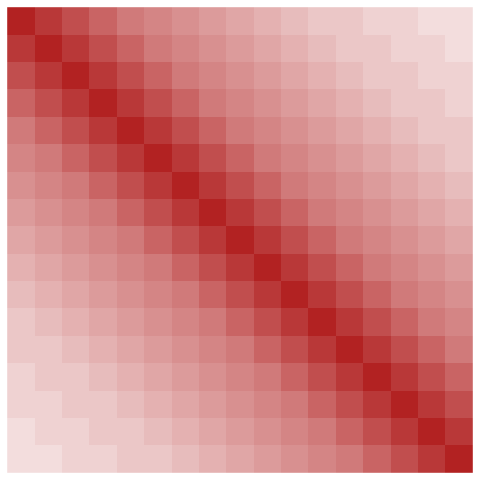
\includegraphics[width = 0.4\textwidth]{./img/chevSimTheory.png} &
      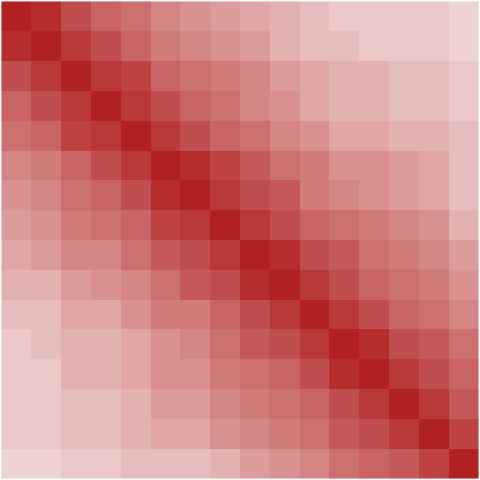
\includegraphics[width = 0.4\textwidth]{./img/chevSim.png} \\
      {\footnotesize (a) Theoretical} &
      {\footnotesize (b) Simulated} \\
    \end{tabular}
  \end{center}
  \caption{The correlation matrices of a population of 500 $F_2$ intercross offspring measured on a 100 cM chromosome with markers each 6.25 cM apart.}
  \label{fig:chevSims}
\end{figure}

Figure \ref{fig:chevSims}(a) displays a pattern of constant off-diagonal lines of decreasing value, as expected from Equation \ref{eq:haldanemap}. Roughly the same pattern is seen in Figure \ref{fig:chevSims}(b), though it is much noisier. Rather than having clear constant lines along each off-diagonal, Figure \ref{fig:chevSims}(b) has regions of similar values which occur across several off-diagonal lines. This leads to the appearance of large squares of more strongly related values, a pattern absent from Figure \ref{fig:chevSims}(a).

\begin{figure}[htp]
  \begin{center}
    \begin{tabular}{cc}
      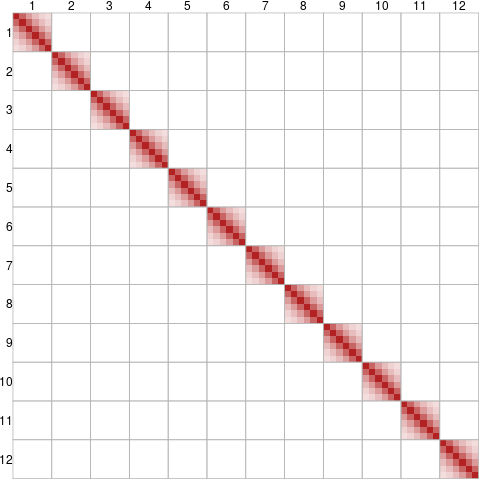
\includegraphics[width = 0.4\textwidth]{./img/LBSimTheory.png} &
      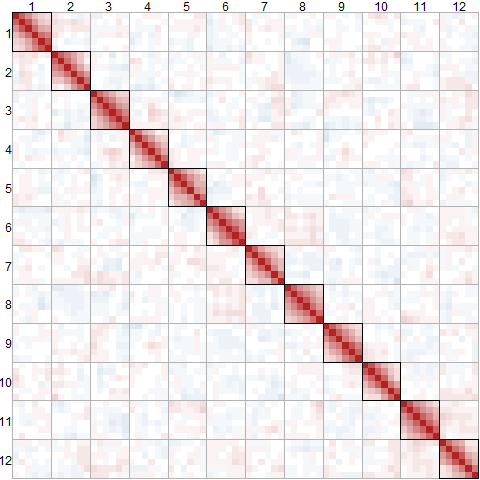
\includegraphics[width = 0.4\textwidth]{./img/LBSim.png} \\
      {\footnotesize (a) Theoretical} &
      {\footnotesize (b) Simulated} \\
    \end{tabular}
  \end{center}
  \caption{The correlation matrices of a population of 250 $F_2$ backcross offspring measured on twelve 100 cM chromosomes with markers 20 cM apart on each.}
  \label{fig:LBSims}
\end{figure}

Figure \ref{fig:LBSims} displays the \cite{LanderBotstein1989} setting with the addition of guide lines to aid in reading the plot. These guide lines extend from labels on the top and left sides of the plot to indicate the chromosome of each marker. These lines create square borders along the diagonal which distinguish the intra-chromosome correlations within their borders from the inter-chromosome correlations outside of them. As suggested by Equation \ref{eq:haldanemap} and shown in Figure \ref{fig:LBSims}(a), Figure \ref{fig:LBSims}(b) has a stark block diagonal structure which agrees with these diagonal squares. The simulation therefore agrees very well with theory in this aspect. Within the chromosomes, there is also good agreement between Figure \ref{fig:LBSims}(a) and Figure \ref{fig:LBSims}(b). Both have decreasing correlations along the off-diagonal lines, with Figure \ref{fig:LBSims}(b) displaying similar departures from Figure \ref{fig:LBSims}(a) as Figure \ref{fig:chevSims}(b) does from Figure \ref{fig:chevSims}(a).

A more interesting noise pattern is seen between chromosomes outside the blocks in Figure \ref{fig:LBSims}(b). Unlike the strictly positive correlations seen in Figure \ref{fig:chevSims}, both negative and positive correlations are observed. Though many chromosomes show consistent patterns between their markers, with all correlations either positive or negative as between chromosomes 9 and 6 or 11 and 12, many have more complicated relationships. Between chromosomes 7 and 3, for example, both negative and positive correlations are observed between markers which are larger than the smallest intra-chromosomal correlations within 2.

%The patterns present in Figures \ref{fig:backsim} and \ref{fig:intersim} are exactly as expected from Section \ref{sec:correlation}. There is an almost perfect similarity between the backcross and intercross design, with only small local variations present between them, in particular for setting (a). All settings show a clear maximum along the main diagonal and a regular decay for off-diagonal elements. Indeed, setting (b) demonstrates how this decay is faster for more distantly spaced markers than nearer ones with its distinct fan pattern. Setting (c) additionally demonstrates the lack of correlation between different chromosomes with its striking block structure for both the backcross and the intercross.

%Such simulations are a confirmation of the earlier analysis performed, but were much more time consuming than using the analytical results. This suggests that the current standard method of simulating large populations is a rather inefficient way of achieving the same result as the analytical prescription of Section \ref{sec:correlation}. Conveniently, the prescription ignores the particular setting: both the backcross and intercross behave identically when viewed through the lens of correlation.

%\subsection{Implementation}

%In order to make the above procedures repeatable, easily read, and flexible, the code for these simulations was implemented in \R using the S3 class system. The core construct was a class meant to reflect $\m{X}$.

%Objects of the \code{genome} class are lists with two elements: \code{alleles} and \code{dists}. The \code{alleles} element is a list of two column matrices, where each matrix represents the value of $\m{X}$ for a particular chromosome. \code{dists} is a list of vectors of the same length as \code{alleles}. Each vector in \code{dists} gives the distances between the alleles in the corresponding element of \code{alleles}. A function called \code{abiogenesis} allows for the convenient creation of a genome through the specification of distances and allele values.

%The function \code{sex} is then used to cross any pair of \code{genome} objects with the use of a \code{meiosis} helper function. \code{sex} accepts an arbitrary distance function which is passed to \code{meiosis} to convert the \code{dists} elements of the \code{genome}s into probabilities of crossing over. By default, the Haldane map distance conversion of Equation \ref{eq:haldanemap} is used. Random Bernoulli trials for each of these probabilities then determines the locations of cross over events, and sections of the columns of \code{alleles} are swapped accordingly.

%The correlation of repeated swaps is then computed via \code{popCorrelation}. As the choice of scoring is at the discretion of the analyst, it accepts not only a list of \code{genome} objects representing the result of repeated crosses, but also a scoring function which accepts a single \code{genome} and returns a $\ve{z}$ value. By default, the additive scoring of $\ve{z} = \ve{x}_1 + \ve{x}_2$ is used.

%The score function generates the $\ve{z}$ values for each \code{genome} provided to \code{popCorrelation}, and correlations between the elements of these $\ve{z}$ are computed. Finally, the \code{image} wrapper \code{corrImg} displays a correlation matrix rearranged so that the main diagonal is consistent with the typical arrangement of correlation matrices. 

\section{Comparing the model to reality} \label{sec:model2real}

Though simulation confirms that population correlations generated under the model of Section \ref{sec:theModel} match the predictions of Equation \ref{eq:zcorr}, the true test of any model must involve empirical measurements. This requires data other than in \cite{LanderBotstein1989} and \cite{cheverud2001}, who only perform simulations.

The Mouse Genome Database (MGD) of \cite{bultetal2019mouse} provides annotation data for more than a dozen mouse populations resulting from crosses of known breeds or \emph{strains}. The database also provides the references needed to determine cM distances between markers measured in these experiments. All of these resources are publicly provided at the Mouse Genome Informatics website: \href{www.informatics.jax.org}{www.informatics.jax.org}.

Considering only those experiments with complete observations leaves several data sets. Two of these investigate an identical population setting: the \emph{BSB mouse cross} of \cite{fisleretal1993bsb}. BSB mice are those resulting from the $F_2$ backcross of the C57BL/6J and {\it Mus Spretus} mouse strains, detailed respectively in \cite{C57BL6J} and \cite{dejageretal2009mspretus}. The first of these crosses is the \emph{JAX BSB} cross of \cite{roweetal1994jaxbsb} and the second is the \emph{UCLA BSB} cross of \cite{welchetal1996uclabsb}. Both the JAX and UCLA BSB cross data were downloaded from \href{http://www.informatics.jax.org/downloads/reports/index.html}{http://www.informatics.jax.org/downloads/reports/index.html}.
% The BSB cross was first introduced in \cite{fisleretal1993bsb} to investigate obesity and since used in research such as \cite{montagutellietal1996epistatic, cheverud2001, watkinsetal2008genomic}.

The data sets require further cleaning before being used, however. First, any markers which do not have a known position along a chromosome in cMs are removed from both data sets. Following that, any individual mice with incomplete data are excluded. For the JAX BSB data this leaves 94 mice annotated at 1496 markers while the UCLA BSB data has 66 mice annotated at 111 markers. The correlation matrices for these data sets are displayed in Figures \ref{fig:jaxbsb}(a) and \ref{fig:uclabsb}(a) respectively.

To determine the expected distribution of these correlations, the cM positions of measured markers were used to simulate 10,000 crosses under each of the JAX BSB and UCLA BSB settings using the methods of Section \ref{sec:sim}. Figures \ref{fig:jaxbsb}(b) and \ref{fig:uclabsb}(b) display example correlation matrices from one such simulated population. For each setting, the quantile of the each experimental pairwise correlation was then computed using the 10,000 simulated crosses. Figures \ref{fig:jaxbsb}(c) and \ref{fig:uclabsb}(c) display those quantiles which are less than 250 in blue and those which are greater than 9,750 in red for their respective settings. These correspond to unadjusted two-sided 95\% confidence rejection regions for each correlation.

\begin{figure}[htp]
  \begin{center}
    \begin{tabular}{ccc}
      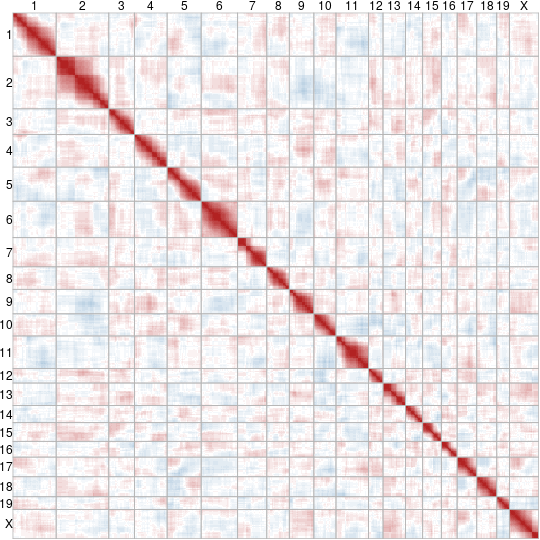
\includegraphics[width = 0.300\textwidth]{./img/jaxbsb.png} &
      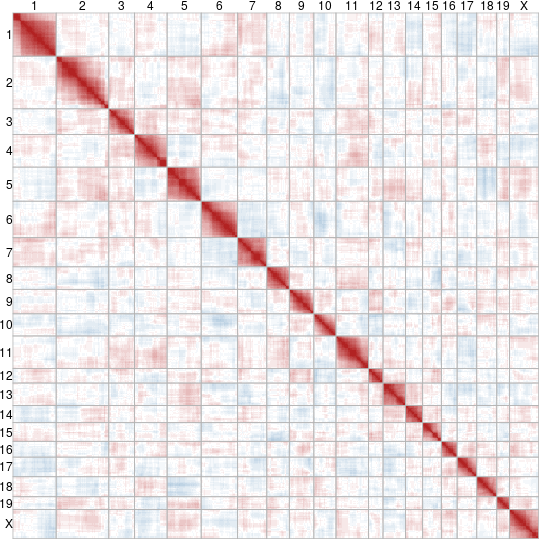
\includegraphics[width = 0.300\textwidth]{./img/jaxbsb_sim.png} &
      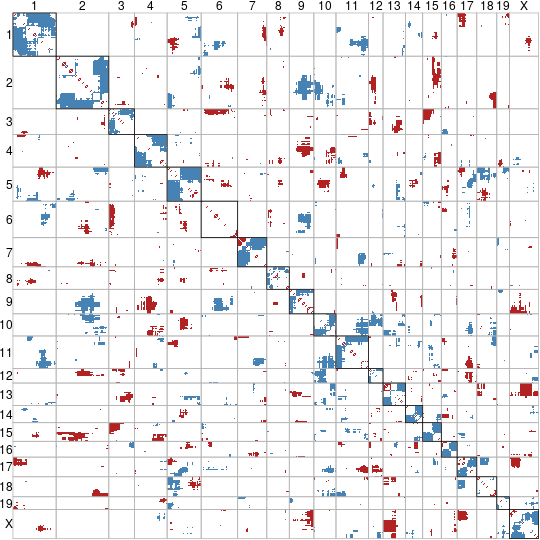
\includegraphics[width = 0.300\textwidth]{./img/jaxbsb_quant.png} \\
      {\footnotesize (a) Experiment} &
      {\footnotesize (b) Simulated example} &
      {\footnotesize (c) Observed quantiles} \\                            
    \end{tabular}
  \end{center}
  \caption{Observed and simulated correlations for the \href{http://www.informatics.jax.org/downloads/reports/MGI_JAX_BSB_Panel.rpt}{MGD JAX BSB cross} from \cite{roweetal1994jaxbsb}. (c) displays quantiles determined from 10,000 simulated crosses, those quantiles less than 250 are shaded blue and those greater than 9,750 are shaded red.}
  \label{fig:jaxbsb}
\end{figure}

\begin{figure}[htp]
  \begin{center}
    \begin{tabular}{ccc}
      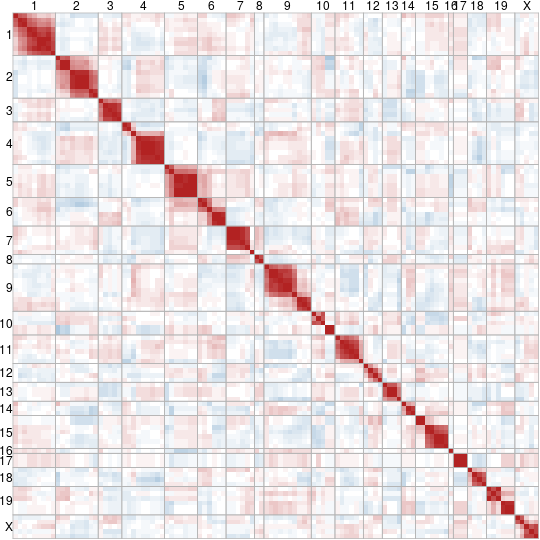
\includegraphics[width = 0.300\textwidth]{./img/uclabsb.png} &
      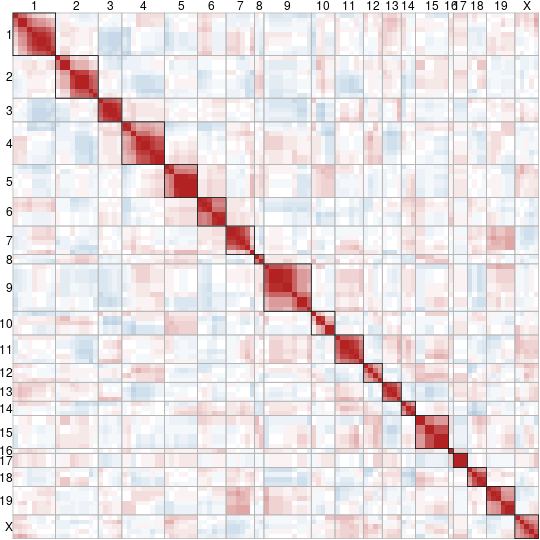
\includegraphics[width = 0.300\textwidth]{./img/uclabsb_sim.png} &
      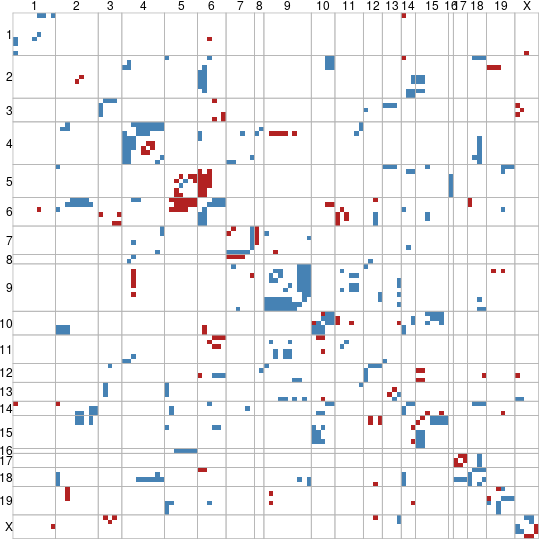
\includegraphics[width = 0.300\textwidth]{./img/uclabsb_quant.png} \\
      {\footnotesize (a) Experiment} &
      {\footnotesize (b) Simulated example} &
      {\footnotesize (c) Observed quantiles} \\
    \end{tabular}
  \end{center}
  \caption{Observed and simulated correlations for the \href{http://www.informatics.jax.org/downloads/reports/MGI_UCLA_BSB_Panel.rpt}{MGD UCLA BSB cross} from \cite{welchetal1996uclabsb}. (c) displays quantiles determined from 10,000 simulated crosses, those quantiles less than 250 are shaded blue and those greater than 9,750 are shaded red.}
  \label{fig:uclabsb}
\end{figure}

Qualitatively, the simulated examples show good agreement to experimental results. In both Figures \ref{fig:jaxbsb} and \ref{fig:uclabsb} the patterns of correlation between chromosomes are similar between experiment and simulation. Figures \ref{fig:jaxbsb}(c) and \ref{fig:uclabsb}(c) additionally suggest that these patterns are little more than noise. The regions of unusually strong correlations shaded in red do not appear to follow any clear pattern, nor do the patterns of unusually weak correlations shaded in blue.

The similarity continues within chromosomes. Figures \ref{fig:jaxbsb}(c) and \ref{fig:uclabsb}(c) are generally not shaded within chromosomes. In particular, very little of the region close to the diagonal is shaded. The most noteworthy pattern in either sub-plot occurs in the corners of the diagonal squares indicating chromosomes in Figure \ref{fig:jaxbsb}(c). Many of these corners are shaded blue, suggesting these distant intra-chromosome correlations are less than might be expected in the JAX BSB cross in many cases. The pattern of shading is suggestive of block structures within chromosomes where contiguous sections are fit well by the model but may have more complex dynamics between them. 

A likely explanation is the non-independence, or \emph{interference}, of cross overs. \cite{bromanetal2002crossover} evaluated the pattern of cross overs in the \cite{roweetal1994jaxbsb} experiment, the basis of the JAX BSB data. Their results suggest that cross overs are not fully independent. Most mouse chromosomes are much less than 100 cM in length, yet cross overs rarely occur within 20 cM of each other and fewer cross overs than expected tend to occur on the same chromosome. This interference will have little impact on the correlation between markers with short distances between them, as more than one cross over event is unlikely to occur in a short interval. Markers separated by longer distances are impacted by this observed interference to a greater extent, as the observed number of double cross overs will be less than expected. This increases chance that distant markers will be separated in meiosis by a single crossover, leading to a weaker correlation than predicted.

That said, it is important not to over-interpret this pattern. It is not repeated in Figure \ref{fig:uclabsb} and the shading of quantiles has not been adjusted to account for the many multiple tests performed in each plot. In order to get a greater sense of this experimental departure from theory, the common markers measured between the UCLA BSB and JAX BSB data were identified and the correlation matrices computed for these common locations. Having two experimental replicates should reduce the impact of one unusual measurement. These correlations are displayed in Figure \ref{fig:bsbcommon}.
\begin{figure}[htp]
  \begin{center}
    \begin{tabular}{cc}
      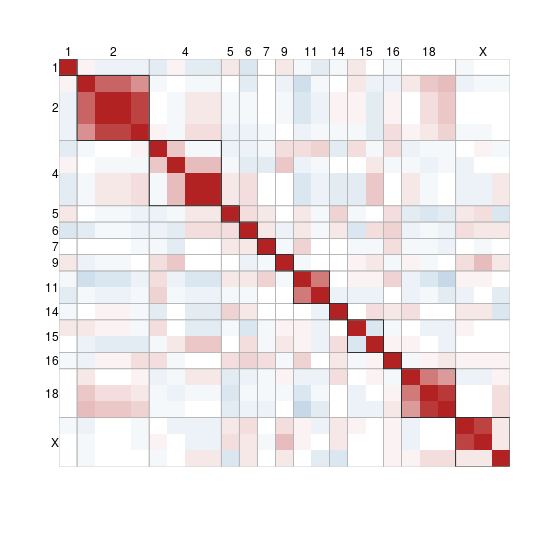
\includegraphics[width = 0.300\textwidth]{./img/jaxbsb_common.png} &
      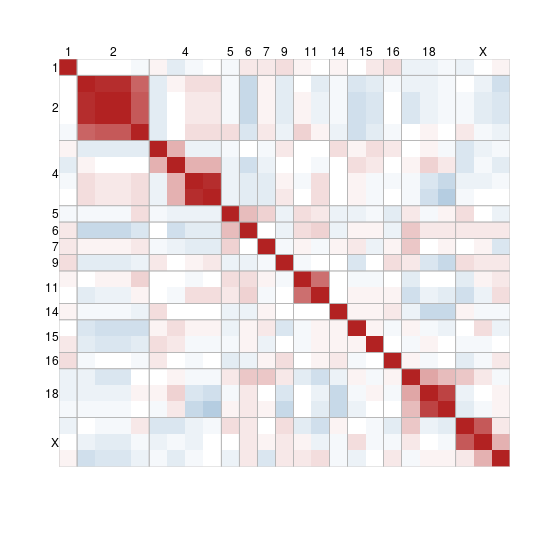
\includegraphics[width = 0.300\textwidth]{./img/uclabsb_common.png} \\
      {\footnotesize (a) JAX BSB cross} &
      {\footnotesize (b) UCLA BSB cross} \\
    \end{tabular}
  \end{center}
  \caption{Observed pairwise correlations for the marker positions measured in both \cite{roweetal1994jaxbsb} and \cite{welchetal1996uclabsb}.}
  \label{fig:bsbcommon}
\end{figure}
Most chromosomes have only one marker measured in common between these experiments, but chromosomes 2, 4, and 18 have several.

A more detailed exploration is given by further simulation. The common markers on chromosomes 2 and 4 were used to generate 10,000 simulated crosses of 80 mice, the average of the JAX and UCLA BSB cross populations. For any pair of markers the resulting distributions can then be compared to the experimental results of \cite{roweetal1994jaxbsb} and \cite{welchetal1996uclabsb} using the two-by-two layouts of Figure \ref{fig:2by2}.

\begin{figure}[htp]
  \begin{center}
    \begin{tabular}{cc}
      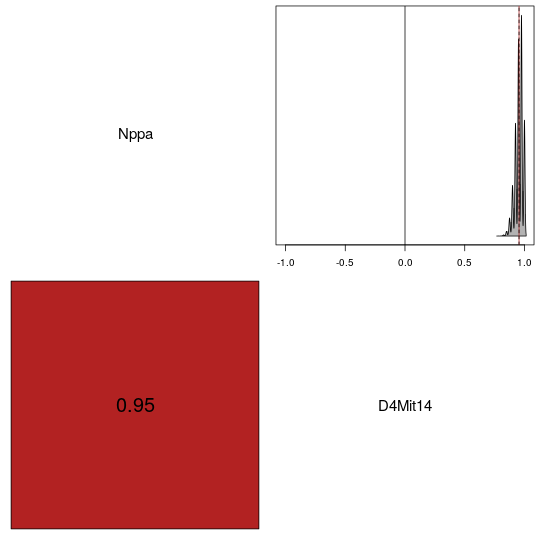
\includegraphics[width = 0.300\textwidth]{./img/bsbCorr2by2.png} &
      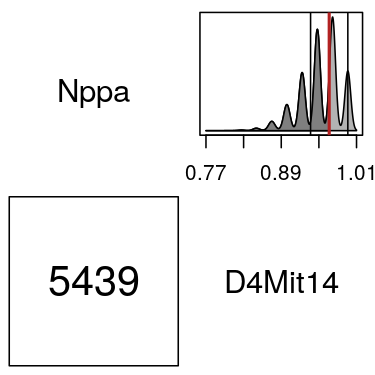
\includegraphics[width = 0.300\textwidth]{./img/bsbCorrTest2by2.png} \\
      {\footnotesize (a) Correlation distribution plot} &
      {\footnotesize (b) Correlation test plot} \\
    \end{tabular}
  \end{center}
  \caption{The correlation plots.}
  \label{fig:2by2}
\end{figure}

Each of the two subplots of Figure \ref{fig:2by2} consists of four cells. Along the diagonal, each cell provides one MGD marker symbol to display the pair of markers being compared. Above the diagonal a distribution is displayed, in both cases the kernel density estimate (KDE) of the correlation over the 10,000 simulated crosses of 80 mice. Below the diagonal a numeric summary with some informative shading is displayed.

Figure \ref{fig:2by2}(a) displays the KDE on a plot reflecting the range of possible correlations in the upper cell and adds a solid black line at the theoretical value predicted by Equation \ref{eq:haldanemap} and dashed red line at the mean over all simulations. The lower cell reports the mean value of these correlations shaded with the divergent palette of Figures \ref{fig:chevSims} to \ref{fig:bsbcommon}.

Figure \ref{fig:2by2}(b) displays the KDE in more detail by placing it in a plot with limits set by the estimate in the upper cell. Two solid lines are added at the correlations computed from the JAX and UCLA BSB data and a thicker red line is added at their mean, below which the density is shaded. The lower cell of Figure \ref{fig:2by2}(b) communicates the quantile of this red line, that is how many simulated correlations fall in the shaded region. As in Figures \ref{fig:uclabsb} and \ref{fig:jaxbsb}, this cell is shaded blue if the quantile is less than 250 and red if it is greater than 9,750.

For the two markers being compared in particular in Figure \ref{fig:2by2}, D2Mit19 and D2Mit22, a number of aspects are of note. Figure \ref{fig:2by2}(a) reiterates the close agreement of simulation and theory. The simulated mean line and the theoretical value are identical at 0.83. This is reasonably consist across all simulations, the KDE shows universally strong, positive correlations above 0.5. Figure \ref{fig:2by2}(b) compares the experimental results to this simulated distribution and finds good agreement between the simulated and experimental values. A more interesting feature to note is the roughness of the kernel density estimate, which suggests a discrete distribution of correlations. It seems the population of 80 mice can have only certain values for the correlation between these markers.

Figure \ref{fig:2by2} can be expanded into a larger display by considering it a single pairwise unit to repeat over a larger array. Consider doing this for all common markers on chromosomes 2 and 4 between the JAX and UCLA BSB data. Along the diagonal, all eight marker symbols are displayed. For any cell, the corresponding pair of markers can be found by tracing along the row and column until the diagonal is reached. Interpretation then follows as in the two-by-two case. In an array, the entire pattern can also be seen at a glance, especially in the lower cells, which can then guide inspection of the upper cells in more detail. Such an expansion of Figure \ref{fig:2by2}(a) gives the \emph{correlation distribution plot} of Figure \ref{fig:bsbcorrDist}, while for Figure \ref{fig:2by2}(b) the \emph{correlation test plot} of Figure \ref{fig:bsbcorrTest} results.

\begin{figure}[htp]
  \begin{center}
      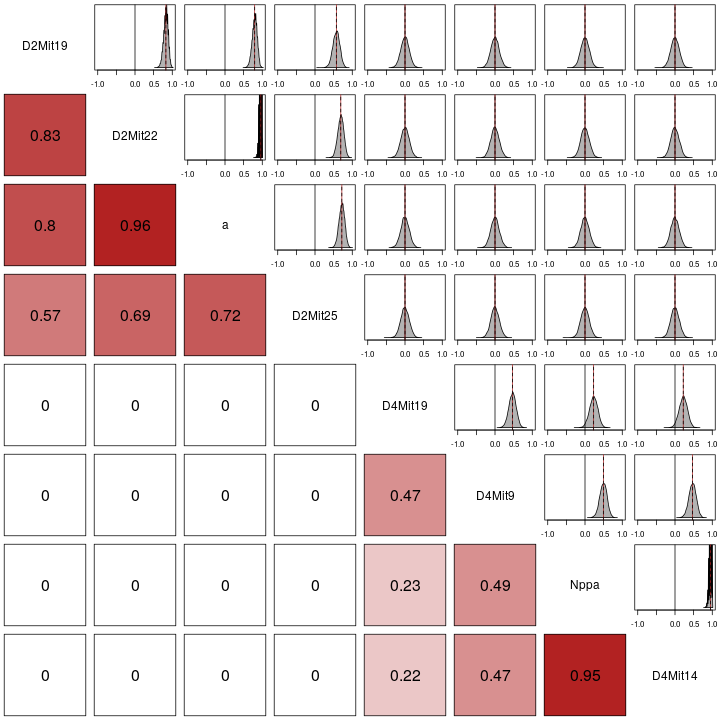
\includegraphics[width = 0.7\textwidth]{./img/bsbCorrDist.png}
  \end{center}
  \caption{The \emph{correlation distribution plot} for the common markers in the JAX and UCLA BSB cross compared to 10,000 simulated BSB crosses.}
  \label{fig:bsbcorrDist}
\end{figure}

In Figure \ref{fig:bsbcorrDist}, the distributions of simulated correlations are all symmetric and unimodal with centres at the theoretical correlation. Indeed, the mean correlation across all simulations agrees with theory to two significant figures for all pairwise correlations. The variation of the distribution seems highly dependent on the proximity of a pair of markers. Markers which are close together and have a high correlation display very little variation across the simulations relative to markers which are further apart on the same chromosome or are independent. Additionally, many of these close markers have a roughness in their KDEs indicative of a discrete distribution. Figure \ref{fig:bsbcorrTest} shows this more clearly.

\begin{figure}[htp]
  \begin{center}
      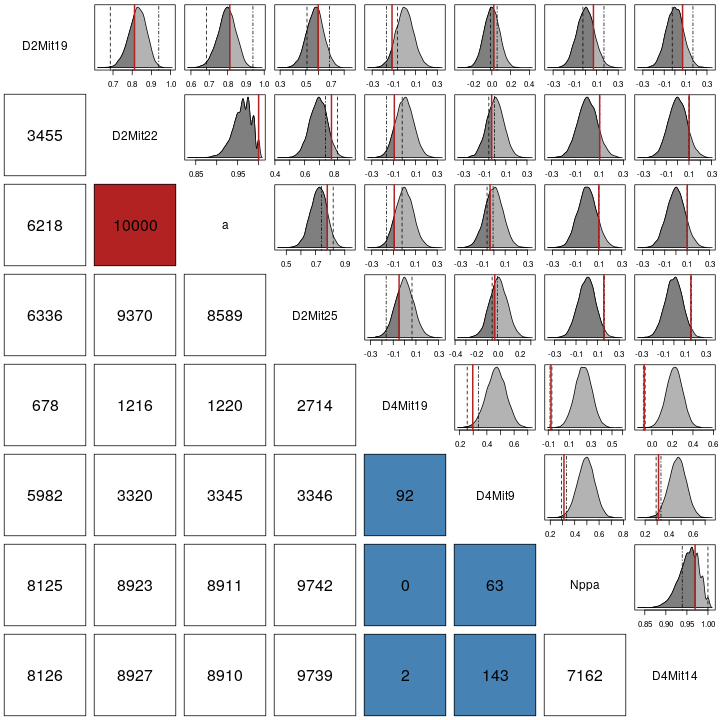
\includegraphics[width = 0.7\textwidth]{./img/bsbCorrTest.png}
  \end{center}
  \caption{The correlation test plot for the JAX and UCLA BSB crosses. The upper cells show the distributions of correlations over 10,000 simulated crosses in detail with both experimental results marked by black lines and their mean marked by a red line. The bottom cells give the quantile of the corresponding mean over the 10,000 simulated crosses.}
  \label{fig:bsbcorrTest}
\end{figure}

The roughness noted in Figure \ref{fig:bsbcorrDist} is one of the defining characteristics of Figure \ref{fig:bsbcorrTest}. In particular the pairs D2Mit22/a and Nppa/D4Mit14 seem to take only seven values across the population. Moreover these values appear to be the same for both pairs. This suggests the correlation for highly associated markers does not take continuous values, but rather can only take one of several values for a population. This is unsurprising when considered in a different light.

As the parents of this cross are known, the correlation is effectively a count of the number of cross overs which have occurred in a population. For highly associated markers only a few are likely to occur. Each peak in the KDEs for the closely related pairs D2Mit22/a and Nppa/D4Mit14 corresponds to hypothetical correlations resulting from no cross overs, one cross over, two cross overs, and so on. For example, the peak at 1 corresponds to populations in which no marker pairs are separated and the peak at 0.975 corresponds to populations with exactly one individual having separated markers. The following peaks at lower values similarly correspond to increasing numbers of individuals with separated markers. This discrete pattern is present in all plots, but the short range and small number of potential values in the case of close associaton leads to the selection of a small bandwidth, therefore accentuating the discrete nature in the KDE. That roughness appears somewhat for moderately close markers supports this.

In the lower cells, the lack of shading suggests close agreement of the model to reality. Only two of the comparisons have means in a rejection region, and both are correlations on chromosome 4. The corresponding cells above the diagonal show much less variation between the JAX and UCLA BSB data than most other cells. Indeed, the two seem to have almost identical correlation values. This suggests that there may be more complexity in chromosome 4 than is captured by the model, potentially due to cross over interference as in Figure \ref{fig:jaxbsb}. This hypothesis is bolstered when chromosome 18 is added in Figure \ref{fig:bsbcorrTestBig}.

\begin{figure}[htp]
  \begin{center}
      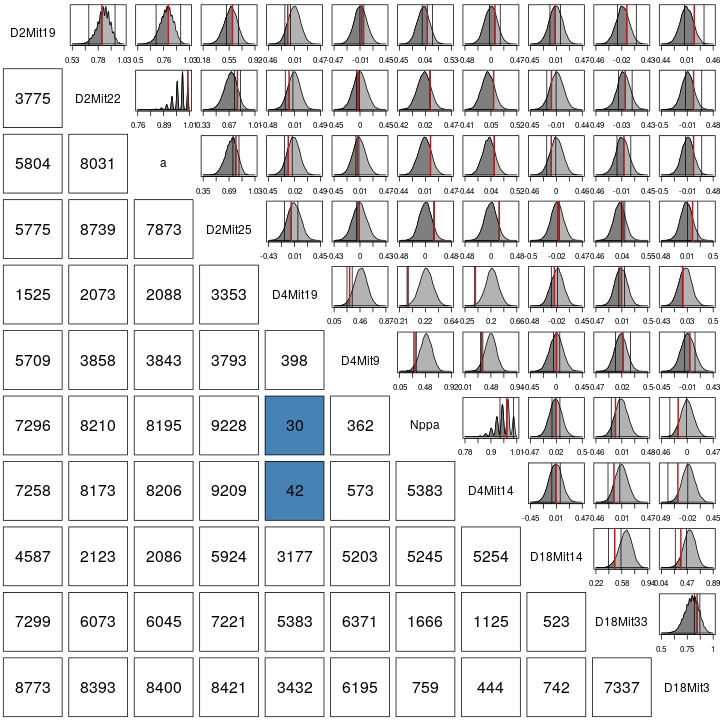
\includegraphics[width = 0.7\textwidth]{./img/bsbCorrTest2.png}
  \end{center}
  \caption{Adding chromosome 18's three common markers to Figure \ref{fig:bsbcorrTest}.}
  \label{fig:bsbcorrTestBig}
\end{figure}

Chromosome 4 is clearly noteworthy for the poorer fit of the model to its correlations than in the case of the other two chromosomes. Compared to chromosomes 2 and 18, there is also reduced variation in the correlations between the two experiments for chromosome 4. This is somewhat harder to read, as both the correlation test plot and correlation distribution plot scale poorly in the number of markers due to the decreasing cell size as the array dimensions grow in a constant figure area.

%\cite{cheverud2001} cites \cite{cheverudetal2001} in which two inbred mouse strains were crossed to breed an $F_2$ intercross population of 510 individuals. It is of particular interest because \cite{cheverud2001} reproduces the correlation matrix of $\ve{z}$ under the additive mapping for the population, providing the opportunity to compare Equation \ref{eq:zcorr} to observed correlations generated from a real cross. Figure \ref{fig:corr2real} displays this comparison.

%\begin{figure}[htp]
%  \begin{center}
%    \begin{tabular}{cc}
%      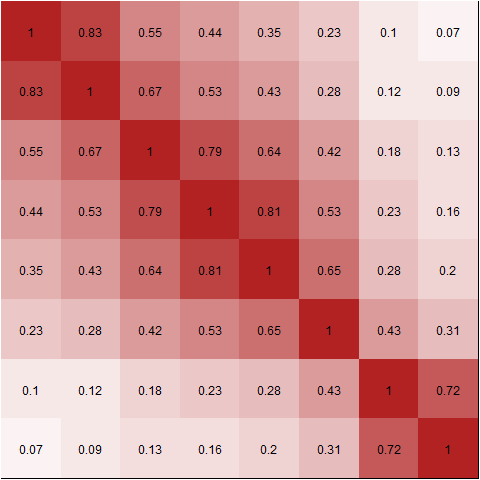
\includegraphics[width = 0.300\textwidth]{./img/chevCorrTheory.png} &
%      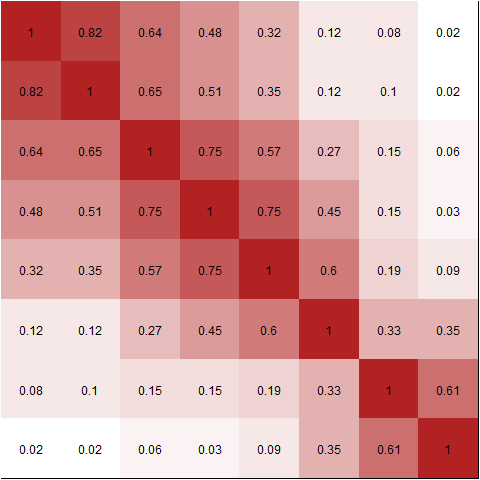
\includegraphics[width = 0.300\textwidth]{./img/chevCorr.png} \\
%      {\footnotesize (a) Theory} &
%      {\footnotesize (b) Experiment} \\
%    \end{tabular}
%  \end{center}
%  \caption{Experimental and theoretical correlation matrices for the $F_2$ intercross population of \cite{cheverudetal2001}.}
%  \label{fig:corr2real}
%\end{figure}

%Just as in the comparison of simulation and theory, the theoretical and experimental matrices look similar structurally. As markers are no longer equidistant, a more complicated structure is seen in Figure \ref{fig:corr2real}(a) than the constant off-diagonal lines of Figure \ref{fig:chevSims}(a). Nonetheless, the general patterns predicted by theory seem to be present in Figure \ref{fig:corr2real}(b), suggesting an agreement between experiment and theory.

%Evaluating this agreement more rigorously requires a distribution of these correlations under the model of Section \ref{sec:theModel}. Rather than make any parametric assumptions and noting the close agreement between theory and simulation in Section \ref{sec:sim}, repeated simulation of the cross of \cite{cheverudetal2001} was used to obtain an empirical distribution of these correlations. 10,000 simulated populations the 510 $F_2$ intercross mice of \cite{cheverudetal2001} were created and the correlation matrices under the additive map computed for each. The resulting 10,000 matrices provide the distribution for each pairwise correlation, which can then be compared to the experimental values.

%\begin{figure}[htp]
%  \begin{center}
%      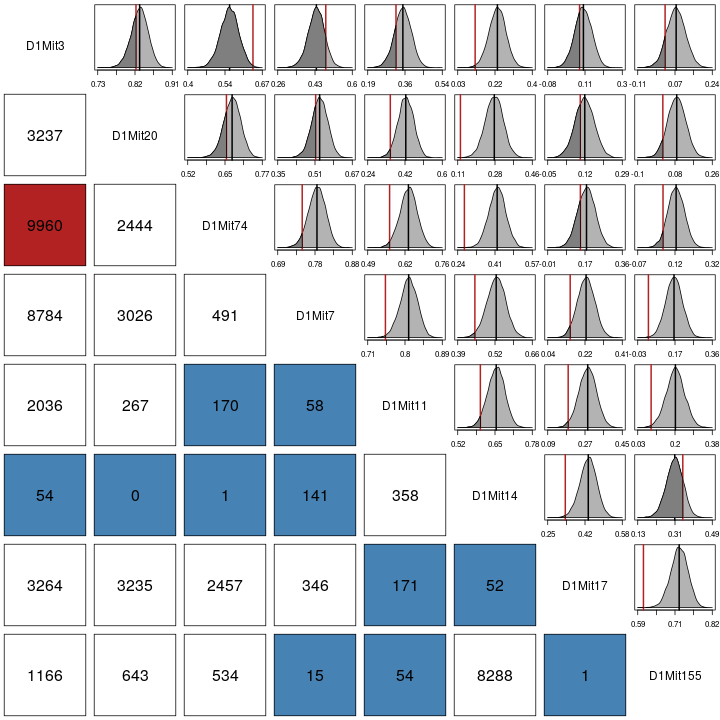
\includegraphics[width = 0.7\textwidth]{./img/chevCorrTest.png}
%  \end{center}
%  \caption{The correlation test plot for data from \cite{cheverudetal2001} compared to simulations under theory.}
%  \label{fig:corrTestPlot}
%\end{figure}

%The \emph{correlation test plot} in Figure \ref{fig:corrTestPlot} was devised to help in this comparison. It is composed of 64 panels arranged in a square array. Each panel above the diagonal displays a kernel density estimate of the distribution of the corresponding pairwise correlation. A black line is added at the theoretical correlation value from Equation \ref{eq:haldanemap} and a red line is added at the correlation value reported in \cite{cheverud2001} and the density is shaded grey outside this line relative to the peak of the density. The names of the markers measured are placed along the diagonal so that the panel in the $i, j$ position of the array represents the correlation between the markers in the $i^{\text{th}}$ and $j^{\text{th}}$ positions along the diagonal.

%Below the diagonal, the number of simulated correlations less than or equal to the experimental correlation for the corresponding pair is displayed. Unadjusted 95\% confidence regions determine the colouring: experimental values greater than 9,750 simulated values or more are shaded red while those greater than or equal to 250 simulated values or less are shaded blue.

%An important insight gained from the correlation test plot is the strong agreement of simulation and theory as shown in the panels above the diagonal. The simulated correlations form symmetric, unimodal distributions centred on the theoretical values for all pairs. Such an observation is a stronger indication of the suitability of the theoretical model than earlier comparisons due to the thousands of repeated simulations performed here. These panels also indicate that the observed correlations are similar to the model, though the model typically overestimates the correlation.

%This observations can be refined using the panels below the diagonal. These make it clearer that the model tends to overestimate compared to the results of \cite{cheverud2001}. All but three of the observed correlations are below the centre of the simulated distribution. Moreover, the extreme values outside of a single test 95\% confidence region are dominantly shaded blue, indicating a value much lower than expected. It is important to note that fewer values would be shaded if these regions were adjusted for the multiple testing implicit in the plot.



%\section{Other views} \label{sec:apply}

%While the development of the model in Section \ref{sec:theModel} focused on heredity from a given father and mother, a radically simplified model can be considered for a population of unknown heritage. Rather than considering the values in $\m{X}$ for an individual in this population in terms of the parental variants, the possible values can, instead, be considered directly when determining the pairwise relationship between two markers.

%Recall the simplified two marker versions of $\m{X}$ from Section \ref{sec:correlation}. Consider a column of $\m{X}$, say $\ve{x}_1$, and note that the two entries of $\ve{x}_1$ only take values in $\{0,1\}$, giving four possible combinations. For every possible combination, there is a corresponding probability of an individual in a population having such a combination on a variant. Suppose these are defined as in Table \ref{tab:r2}.

%\begin{table}[!ht]
%  \centering
%  \begin{tabular}{c c| c c| c}
%    & \multicolumn{1}{c}{} & \multicolumn{2}{c}{$x_{11}$} & \\ \cline{3-4}
%    & & 0 & 1 & \underline{Marginal} \\ \cline{2-4}
%    \multirow{2}{*}{$x_{21}$} & \multicolumn{1}{|c|}{0} & $p_{ab}$ & $p_{Ab}$ & $1-p_B$ \\
%    & \multicolumn{1}{|c|}{1} & $p_{aB}$ & $p_{AB}$ & $p_B$ \\ \cline{2-4}
%    & \multicolumn{1}{c}{Marginal} & \multicolumn{1}{c}{$1 - p_A$} & \multicolumn{1}{c}{$p_A$} &  \\ 
%  \end{tabular}
%  \caption{Probabilities of combinations of $\ve{x}_1$ in a population of individuals.}
%  \label{tab:r2}
%\end{table}

%This conceptualization, which does not directly consider the parentage of a population, is dominant in the literature.

%\subsection{Settings in the Literature} \label{subsec:inlit}

%Despite this difference, the settings introduced in Section \ref{subsec:sim} occur commonly in the literature. Among studies focusing on real data, including \cite{Galwey2009}, \cite{nyholt2004}, and \cite{Salyakina2005}, the structure of selected markers is motivated by previous work. As a consequence, these studies typically only view one chromosome, indeed one small section of a chromosome, associated with a phenotype. Additionally, the markers within this segment are typically not evenly spaced, a situation similar to setting (b) from Section \ref{subsec:sim}. Typically, these distances are not reported in centimorgans, but instead in base pairs.

%In contrast, simulation studies seem to be characterized by equidistant measurements on one or several chromosomes. \cite{cheverud2001} performs simulation on a single chromosome with equidistant markers, and records the results for several distances. This is of the same form as setting (a) from Section \ref{subsec:sim}. \cite{LanderBotstein1989} examines a case of 12 chromosomes with markers spaced every 20 cM along each, which is a specific case of setting (c).

%Departing from a reference to distances in centimorgans or base pairs, \cite{LiJi2005} set their simulation scenarios using the genetic $r^2$ measure, defined by \cite{hillrobertson1968} as

%\begin{equation} \label{eq:rsq}
%  r^2 = \frac{\left ( p_{AB} p_{ab} - p_{Ab} p_{aB} \right )^2}{{p_A (1 - p_A) p_B (1 - p_B)}} = \frac{\left ( p_{AB} - p_A p_B \right )^2}{p_A (1 - p_A) p_B (1 - p_B)},
%\end{equation}

%\noindent which is exactly Pearson's product moment correlation for the two by two contingency table case. In adopting this measure to define their simulation settings, \cite{LiJi2005} use different language than other studies. Their simulation is described as an investigation of ten independent regions within which five markers are placed such that adjacent markers have an $r^2$ of 0.8 between them. Despite this difference in language, this design is clearly analogous to setting (c) from Section \ref{subsec:sim}.

%The use of $r^2$ by \cite{LiJi2005} to specify their population parameters is somewhat curious, however. $r^2$ presents difficulties for measuring genetic distance over generations in any model including recombination. Consider $p_{AB}$, $p_A$, and $p_B$ and their relationship over generations. Without selection in survival or mating, $p_A$ and $p_B$ will remain constant, while $p_{AB}$ will change.

%Suppose we have an offspring with
%$$\m{G} = \begin{bmatrix}
%  1 & g_{12} \\
%  1 & g_{22} \\
%\end{bmatrix}.$$
%There are two possibilities for $\m{M}$ which could result in this particular $\m{G}$ when the independence of variant heritability is considered:
%$$\m{M} = \begin{bmatrix}
%  1 & g_{12} \\
%  1 & g_{22} \\
%\end{bmatrix}, \text{ or }
%\m{M} = \begin{bmatrix}
%  g_{11} & 1 \\
%  1 & g_{22} \\
%\end{bmatrix}.$$
%In the first of these two $\m{M}$ configurations, $\m{G}$ results if no recombination occurs, while in the second $\m{G}$ results if recombination occurs. The first configuration occurs with probability $p_{AB}$ and is passed on with probability $1 - p_r(d)$, as recombination disturbs the necessary variant. The second configuration occurs with probability $p_Ap_B$ and is passed on with probability $p_r(d)$.

%Denoting $p_{AB,k}$ as the value of $p_{AB}$ at generation $k$, we then write

%$$p_{AB,k} = [1 - p_r(d)] p_{AB,k-1} + p_r(d) p_A p_B,$$

%\noindent from which it can easily be derived that

%$$r^2_k = \left [ 1 - p_r(d) \right ]^2 r^2_{k-1} =  \left [ 1 - p_r(d) \right ]^{2k} r^2_0$$

%\noindent and so

%$$\lim_{k \rightarrow \infty} \left [ 1 - p_r(d) \right ]^{2k} r^2_0 = 0$$

%\noindent whenever $p_r(d) > 0$.

%In this manner, strongly associated markers $A$ and $B$ become less associated over time in the absence of selection pressures in sexual reproduction and survival, as noted in \cite{siegmundyakir2007}. This makes the use of $r^2$ under any model with recombination problematic, as its use requires the specification of an initial condition and generation of interest. \cite{LiJi2005} simulate data using given $p_A$, $p_B$, and $r^2$ values to determine $p_{AB}$ and generate a population which matches $p_A$, $p_B$, and $p_{AB}$. This method therefore ignores the population characteristics of the parents and offspring, instead providing only a snapshot of the population characteristics at a particular time.

%It is therefore far more natural to use a distance in these studies. Whether reported in centiMorgans, base pairs, or some other measure, these measures remain constant over generations, and govern the dynamics of recombination.

\section{Conclusion} \label{sec:conclusion}

Despite this, many of the introductions to the field rely on the models of early pioneers of genetics. The works of Mendel, Pearson, Fisher, Haldane, and others in genetics were groundbreaking, but also occurred well before a modern understanding of DNA or the mechanics of inheritance \cite{visschergoddard2019}. As a result, these models do not provide a modern context. Modern textbooks and papers consequently introduce the structure of DNA and the models describing inheritance in separate sections, if the structure of DNA is addressed at all \cite{crowkimura1970intro, siegmundyakir2007, xu2013principles, liu1998statistical}. Such complete and detailed accounts with the biology and statistics separated are unquestionably important, but fail to present an accessible and unified picture of genomics for researchers with a statistical background. \TODO{Move to conclusion: ``this model provides a map to help understand larger works''}

\cite{laframboise2009} notes that microarrays remove the middle steps entirely: by taking luminance directly it is possible to inspect and relate $\ve{z}$ to physical characteristics without subjective intermediate steps.

This framework may not be limited to genomics. \cite{hasinetal2017multi} note the expansion of genome-wide methods to protein and RNA sequencing. In both of these cases, the framework above applies, but has less explanatory power. One might imagine investigating proteins using this framework to see which are relatively under or over-expressed

Each of these italicized steps could be performed in a number of ways, with consequences on the final quantification of the genome's relevant features. Selection typically involves the choice of at most one million SNPs from an SNP database such as \cite{NCBIdbSNP}. Though these databases have hundreds of millions of identified SNPs, \cite{koboldtetal2013next} suggests that perhaps only 15 million are common enough to be useful, and that no further useful SNPs are likely to be found. While modern microarray technology dictates the limit on the number of simultaneously selected SNPs, see \cite{laframboise2009, tametal2019benefits}, studies such as \cite{assimesetal2016cadgwas} often choose far fewer. These rely on SNPs used in previous literature and ready-made general microarrays as selection criteria. \cite{LanderBotstein1989} proposes SNPs selected uniformly across the genome for agnostic studies.

There are new technologies which allow entire genomes to be sequenced, see \cite{heatherchain2016sequencers, hasinetal2017multi, uffelmannetal2021gwas}, but even when these reach a cost and speed accessible to most researchers there is little doubt known markers with previous literature will still be the focus of many studies. These technologies are more likely to expand the selection pool than to make selection irrelevant.

Categorical measures of association, such as the $\chi^2$ test, could readily be applied to $\m{T}$, where each possible row combination is treated as a different category. Such measurement would likely be more computationally inefficient, but would entirely circumvent the last two steps of Figure \ref{fig:modelDiagram}. 


\bibliographystyle{plainnat}
\renewcommand*{\bibname}{References} % use title "References" for bibliography
\bibliography{../Bibliography/fullbib}

\end{document}
